\documentclass[a4paper]{article}

\usepackage[utf8]{inputenc}    % enables use of utf8 characters in the input file
\usepackage[T1]{fontenc}       % enables proper output of unicode characters such that text can be copy-pasted from the pdf file
\usepackage{hyperref}          % enables pdf index, links for web addresses, intra-document links
\usepackage{a4wide}            % reduces page margins
\usepackage{parskip}           % replaces hanging paragraphs with spacing between paragraphs
\usepackage{times}             % replaces Computer Modern font with something resembling Times
\usepackage{graphicx}          % enables including graphics
\usepackage{caption}           % provides float caption formatting
\usepackage{subcaption}        % provides subfloat functionality and caption formatting
\usepackage{amsmath}           % ams math module
\usepackage{amssymb}           % ams math symbols
\usepackage{mathtools}         % fixes a few quirks with the ams packages

% functions
\DeclareMathOperator{\atan2}{atan2}
\DeclareMathOperator*{\argmin}{argmin}
\DeclareMathOperator*{\argmax}{argmax}

% braces
\newcommand{\xp}[1]{\left(#1\right)}   % parentheses
\newcommand{\xb}[1]{\left[#1\right]}   % brackets
\newcommand{\xc}[1]{\left\{#1\right\}} % curly braces
\newcommand{\xa}[1]{\left|#1\right|}   % absolute value
\newcommand{\xn}[1]{\left\|#1\right\|} % vector norm

% types
\newcommand{\function}[2]{#1 \rightarrow #2}
\newcommand{\R}[1]{\mathbb{R}^{#1}}
\newcommand{\RR}{\mathbb{R}}
\newcommand{\unit}{\xb{0,1}}

% complex terms
\newcommand{\apply}[2]{#1\!\xp{#2}}
\newcommand{\integral}[4]{\int_{#1}^{#2} #3 \; \mathrm{d}#4}
\newcommand{\powerset}[1]{\apply{\mathcal{P}}{#1}}

% continuity
\newcommand{\contp}[1]{\mathrm{C}^{#1}}
\newcommand{\contg}[1]{\mathrm{G}^{#1}}

% vectors
\newcommand{\vectorA}[1]{\begin{pmatrix}#1\end{pmatrix}}
\newcommand{\vectorB}[2]{\begin{pmatrix}#1\\\linebreak{}#2\end{pmatrix}}
\newcommand{\vectorC}[3]{\begin{pmatrix}#1\\\linebreak{}#2\\\linebreak{}#3\end{pmatrix}}
               % some math helper macros

% tells LaTeX to avoid orphan lines at the beginning or end of a page
\clubpenalty = 10000
\widowpenalty = 10000

% setup caption formatting
\captionsetup{margin = 10pt, font = small, labelfont = bf}

\title{Optimal Fitting of Planar Curves to Prescribed Constraints}
\author{Julian Asamer, Julian Brunner}
\date{February 13, 2014}

\begin{document}

	\maketitle

	\begin{abstract}

		\noindent We analyze the usability of curve design tools in current vector graphics software and suggest an abstract approach for designing improved, usability-oriented tools. We instantiate this approach using a powerful description language and the minimum variation curve fairness measure on top of nonlinear optimization on polynomials, developing a prototype curve design tool in the process. We evaluate our approach and its instantiation based on the prototype and suggest ideas for further research and development.

	\end{abstract}

	\section{Introduction}
	\label{section:introduction}

		These days, vector graphics are widely used in both artistic and industrial design. Artists create illustrations, character designs and even fully animated cartoons using vector graphics software. Vector graphics are also used in industrial design, allowing for the smooth, aerodynamic shapes observed in modern cars and airplanes.

		Raster graphics images (for instance, digital photos and most digitally painted artworks) consist of a finite number of pixels (picture elements) which discretely specify the colors of points on the image. In contrast, vector graphics designs consist of primitives like curves and surfaces, which describe the shapes present in the design using mathematical functions. This has various advantages over the raster approach, since designs do not suffer from discretization artifacts and can, for instance, be arbitrarily scaled and repeatedly modified without any loss of quality.

		The scope of this project is restricted to two-dimensional vector graphics, but many ideas can be applied to three-dimensional vector graphics as well. All elements in two-dimensional vector graphics are described in terms of curves, so the design process of curves is the single most important part of two-dimensional vector graphics. Unfortunately, designing curves using the tools available in current vector graphics software can be very frustrating, with the user being unable to achieve the desired curve shape. To make matters worse it is often unclear why this is the case, as the software seems to put all the necessary tools into the hands of the designer, yet at times, they somehow do not allow the user to communicate their intention to the software.

		While there has been some promising research into improving curve design tools \cite{thesis-mvc} \cite{thesis-spiro}, it focuses mostly on the aspect of improving the fairness of curves, rather than usability as a whole. Additionally, it has not had much of an impact on actual vector graphics software used in practice, which continues to focus almost exclusively on Bézier splines to this day.

		Thus, the objective of this project is to identify the exact nature and cause of the shortcomings of current curve design tools in order to use this knowledge to develop better ones.

	\section{Problem Analysis}
	\label{section:problem_analysis}

		When trying to improve something, it seems advisable to take a step back and thoroughly research the causes of its perceived shortcomings in order to find a way to improve it without making the same or similar mistakes. In the context of curve design tools, this can be achieved by analyzing and modeling the process that people use when designing curves. Once such a model has been obtained, it can be used to propose criteria for good curve design tools as well as to analyze usability aspects of existing tools.

		\subsection{Curve Design Process}
		\label{section:curve_design_process}

			Observing the process that most people seem to go through when designing curves using vector graphics software, the following model appears plausible:
			\begin{enumerate}
				\item obtain the source curve as either a real or a mental image of the curve
				\item extract some properties from the source curve
				\item provide these properties to the software
				\item have the software derive the most likely result curve from these properties
			\end{enumerate}

			Steps 2 to 4 are then repeated on portions of the curve in order to make small adjustments until the result curve is sufficiently similar to the source curve.

			Step 1 is of course independent of any software that may be used by the designer. Step 2 and 3 are strongly influenced by the choice of design tool, as the software dictates which properties it uses for the specification of curves (the specification language the software uses). Unless the properties the designer conveyed to the software in step 3 uniquely identify the curve, in step 4, the design tool will have to choose the curve that the user was most likely describing from a possibly infinite set of curves that exhibit the supplied properties. This notion of `most likely' is usually modeled in terms of a fairness measure, fairer curves being regarded as more likely. Fairness usually encodes intuitive notions such as smoothness and minimality using mathematical concepts such as continuity and variation of curvature. At this point, the software has another opportunity to influence the design process both positively and negatively depending on what fairness measure is chosen as well as the ability of the software to find a curve that has a high fairness.

			Note that there may be multiple ways to describe a given curve design tool in terms of this process. Instead of modeling the selection of the most likely curve using some fairness measure, one may also propose an alternate view on the process in which the user implicitly specifies the exact curve they want in the properties they specify. For example, in a curve design tool which takes two points from the user and connects them using a straight line, one possible view is that the user provides the start and the end point of the curve, and the fairness measure is designed to always select the straight line as the fairest curve. Another way of looking at this process is to say that the user, by supplying \(p_0\) and \(p_1\), specified the coefficients of the linear term \(p_0 + \xp{p_1 - p_0} t\), thus uniquely identifying the desired curve. Modeling the process in such a way that the user supplies only the minimum amount of implicit information, relying on the fairness measure for everything else, is usually closer to reality when analyzing usability of some curve design tool.

			In a similar fashion, one may attribute certain shortcomings (for instance, insufficient continuity) to either the specification language (the language does not allow the user to request curvature continuity) or the fairness measure (the fairness measure does not select sufficiently smooth curves). These decisions have to be made on a case by case basis, selecting the approach that is better suited to modeling the reality of curve design.

		\subsection{Usability Criteria for Curve Design Tools}
		\label{section:usability_criteria_curve_design_tools}

			We conclude that the two ways in which curve design tools can affect the design process, are through their choice of specification language and fairness measure, as well as their practical ability to derive curves from specifications and the fairness measure. Note that while syntactically complete, the semantics of the specification language also depend on the fairness measure. Thus, it makes sense to consider the combination of a specification language and a fairness measure, which will be called a description language.

			Ideally, the description language should be very expressive, yet easy to handle for humans, enabling the user to communicate their intent to the software efficiently. The fairness measure should capture the intuitive notion of curve smoothness sufficiently well and select curves that are minimal with respect to the given specification. These goals are competing with the software's ability to derive curves from descriptions reliably and efficiently, a process which becomes increasingly difficult with more expressive specification languages and more complex fairness measures.

			From these considerations, we think that applying the following criteria is a good start for assessing the usability of curve design tools:
			\begin{enumerate}
				\item expressiveness of the description language
				\item human ability to `read' the specification language from curves
				\item human ability to `speak' the specification language to the software
				\item smoothness of curves selected by the fairness measure
				\item minimality of curves selected by the fairness measure
				\item ability of the software to derive curves from descriptions
			\end{enumerate}

		\subsection{Existing Curve Design Tools}
		\label{section:existing_curve_design_tools}

			Using the model of the curve design process as well as the criteria for usability of curve design software that were established in sections \ref{section:curve_design_process} and \ref{section:usability_criteria_curve_design_tools}, some curve design tools available in common vector graphics software are analyzed.

			\subsubsection{Bézier Splines}
			\label{section:bézier_splines}

				Bézier splines are probably the most widely used type of curve in two-dimensional vector graphics. Bézier splines are defined piecewise using Bézier curves, which are parametric plane curves (see also sections \ref{section:parametric_curves} and \ref{section:parametric_plane_curves}) realized using polynomials in Bernstein form. Cubic Bézier curves are the most frequently used ones. A Bézier curve \(\phi\) of degree \(n\) consists of \(n + 1\) coefficients \(c_i \in \R{2}\), called coefficient points. The curve will always go through the first and the last coefficient point (\(\apply{\phi}{0} = c_0, \apply{\phi}{1} = c_n\)) and stay within the convex hull of the coefficient points at all other times. Bézier curves in a Bézier spline are usually pieced together such that the resulting spline's tangent direction along the curve is continuous.

				In existing vector graphics software, Bézier splines are edited by more or less directly modifying the coefficient points of the underlying Bézier curves. In the case of cubic Bézier curves, the first and the last coefficient points represent the curve's start and end points, while the differences between the second and the first as well as the fourth and the third coefficient points are proportional to the velocity of the curve at the start and end points, respectively. In that sense, the user can specify start end end points of the curve, as well as start and end velocities of the curve using the coefficient points. Most vector graphics tools have functions that allow preserving the directional continuity of the spline by automatically modifying adjacent coefficient points accordingly. They usually do not ensure curvature continuity though. Some tools can also modify existing coefficient points in such a way that the curve passes through a point that is chosen by the user without adding more segments to the spline.

				When applying the model introduced in section \ref{section:curve_design_process} to Bézier spline design tools, there are two possibilities for modeling the fairness measure. One way to view things is to assume that the user, in supplying the four coefficient points of each curve segment, uniquely specifies each segment's Bézier curve and thus the entire spline, leaving no room for choosing a curve according to some fairness measure. Since users usually do not think about Bézier splines that way, it is more practical to assume that the user only supplies both point and velocity at the start and end of each curve segment, with a fairness measure designed to always choose the cubic Bézier curve that is uniquely specified by the given properties as the fairest curve.

				Applying the criteria established in section \ref{section:usability_criteria_curve_design_tools}, we conclude that the design tools for Bézier splines work sufficiently well in terms of humans trying to read and/or speak their specification language (criteria 2 and 3), a skill that can be acquired with some practice. The curve chosen by the fairness measure is reasonably minimal (criterion 5), as the spline's complexity is limited by the number of segments that are used, which is in direct correspondence with the specification. Bézier splines are furthermore very simple to derive from their description, fulfilling criterion 6 perfectly. We think that design tools for Bézier splines have some issues with both the fairness measure's smoothness (criterion 4) and the expressiveness of the description language (criterion 1), both of which shall be analyzed in the following paragraphs.

				The issue with the fairness measure is that it always selects the uniquely determined cubic Bézier curve for each segment, thus not guaranteeing curvature continuity across segments. It is difficult for humans to choose the coefficient points in such a way that curvature continuity is established, making it hard to create smooth curves if the design software does not support the user in this regard. The problem is aggravated by the fact that curvature discontinuities can be hard to spot and may thus only be discovered much later in the design process, increasing the cost of these mistakes. In case the software does support the user by allowing them to request curvature continuous Bézier splines, this sacrifices some degree of freedom for each node, thus restricting the way nodes can be manipulated and in turn possibly forcing the user to place more nodes in order to get the desired result. Placing more nodes leads to some disadvantages that will be discussed further in the next paragraph.

				The description language used to specify Bézier splines in common design tools lacks expressiveness. Specifically, describing curves in terms of their curvature is difficult since curvature may only be specified indirectly through the magnitude of the velocity values (higher velocity resulting in lower curvature). Unfortunately, this is also very dependent on the point and velocity coefficients at the other end of the spline segment. Additionally, there is no way to directly specify constant or linearly changing curvature. This makes specifying curvature very tedious, and in case the winding angle of the curve segment is large enough, actually impossible, forcing the designer to use additional nodes in order to achieve the desired result. Using an excessive number of nodes makes it more tedious and time-consuming for the designer to create and/or modify such curves, as many nodes and handles have to be created or moved in order to change the overall curve. It also sacrifices smoothness, since it is easy to accidentally introduce subtle bumps in the curve when using a large number of nodes. Another issue is that without software support for curvature continuity, using more nodes usually also introduces more points where curvature is not continuous. In cases where the curvature is an important property of the curve (for example the constant curvature of circular arcs, or the linearly changing curvature of spirals), it may be very difficult to specify these properties indirectly using the coefficient points.

				\begin{figure}[htb]
					\centering
					\begin{subfigure}[b]{\textwidth / 1}
						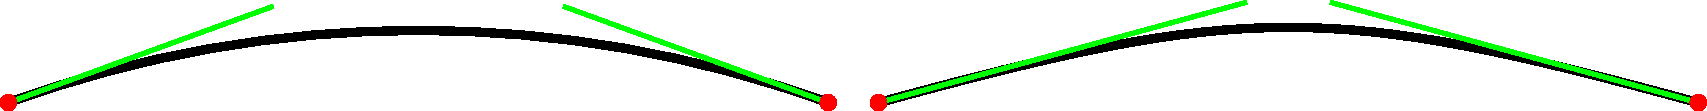
\includegraphics[width=\textwidth]{content/output/examples_bezier_arc.pdf}
						\caption{Circular Arc}
						\label{figure:examples_bézier_arc}
					\end{subfigure}
					\begin{subfigure}[b]{\textwidth / 2}
						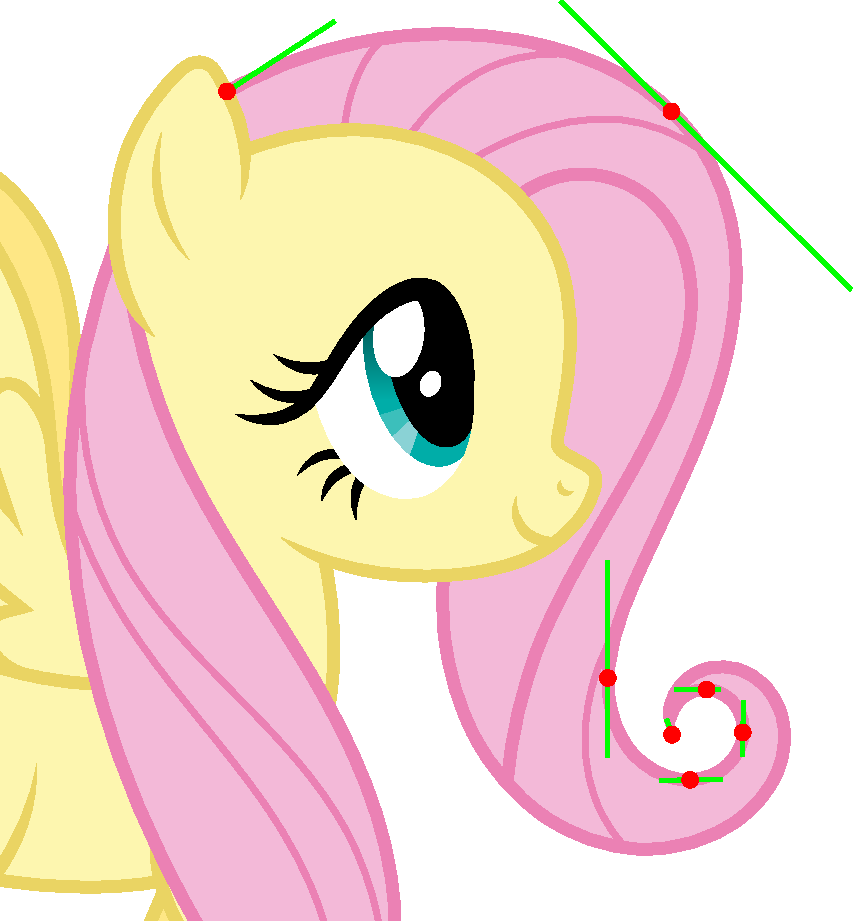
\includegraphics[width=\textwidth]{content/output/examples_bezier_fluttershy.pdf}
						\caption{Fluttershy \cite{fluttershy}}
						\label{figure:examples_bézier_fluttershy}
					\end{subfigure}%
					\begin{subfigure}[b]{\textwidth / 2}
						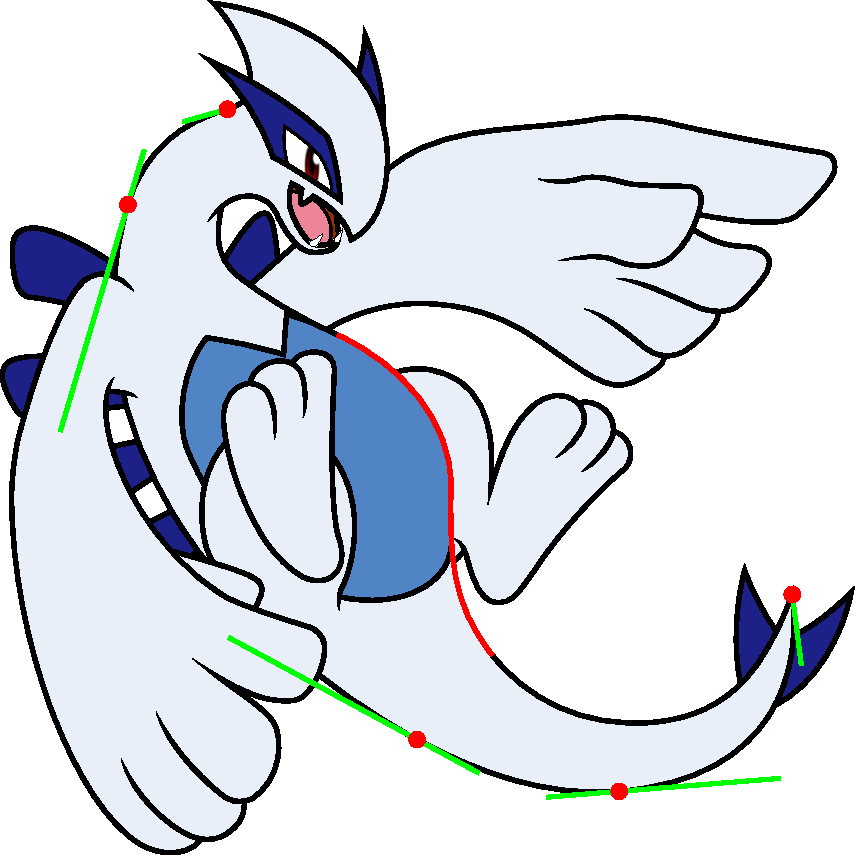
\includegraphics[width=\textwidth]{content/output/examples_bezier_lugia.pdf}
						\caption{Lugia \cite{lugia}}
						\label{figure:examples_bézier_lugia}
					\end{subfigure}
					\caption{Bézier splines, as they appear in common curve design tools. Bézier nodes are displayed as red dots, Bézier handles are displayed as green tangent lines.}
					\label{figure:examples_bézier}
				\end{figure}

				Figure \ref{figure:examples_bézier_arc} shows two Bézier splines. The left curve is a Bézier spline approximation of a circular arc, exhibiting nearly constant curvature, while the right one is not, changing from low curvature to high curvature and back to low curvature. As the difference can be hard to see, it is easy to make mistakes when trying to approximate circular arcs using Bézier splines.

				Figures \ref{figure:examples_bézier_fluttershy} and \ref{figure:examples_bézier_lugia} show curves that could be described more efficiently in terms of curvature. Since there is no way to directly specify curvature using Bézier splines, a considerable number of nodes is needed to get close to the desired curve. This, in turn, makes the curve hard to create and/or modify and may lead to decreased smoothness as discussed in the previous paragraphs.

				The red curve segment in figure \ref{figure:examples_bézier_lugia} is a Bézier spline with a curvature discontinuity which went unnoticed by the artist at the time of creation. In fact, this discontinuity would be even less visible if the curve was not vertical at said point, manifesting itself only in a reduced overall smoothness of the curve, without a clear indication of the problem's origin.

			\subsubsection{Spiro Splines}
			\label{section:spiro_splines}

				Spiro splines \cite{thesis-spiro} were added to Inkscape in 2009. Even though they were integrated using path effects and thus have a somewhat cumbersome user interface, they constitute a commendable effort of incorporating results from curve research into vector graphics software, something that has hardly happened this far.

				Spiro splines consist of parts of the Euler spiral, which is a curve whose curvature changes linearly with the curve's arc length. The user can specify control points through which the software puts an interpolating spline. There is no way to directly specify tangent angle and/or curvature. The splines are guaranteed to have curvature continuity.

				In order to evaluate the usability of Spiro splines, the model from section \ref{section:curve_design_process} is applied once more. In the case of Spiro splines, the modeling is fairly straightforward. The user supplies a set of points for which the software computes an interpolating spline. The fairness measure chooses the segments of this spline to be parts of the Euler spiral, ensuring curvature continuity and trying to avoid excessive winding.

				We analyze Spiro splines in terms of the criteria presented in section \ref{section:usability_criteria_curve_design_tools}. With the specification language of Spiro splines consisting of points on the curve, plus the fact that on sufficiently smooth curves, not very many of them are needed, the language is well-suited to be read and spoken by humans (criteria 2 and 3). The fairness measure leads to beautifully smooth curves that are usually sufficiently close to what a human would expect given the control points (criteria 4 and 5). The software is also reliable and quick with the construction of these curves. There are some cases where the algorithm fails to find a meaningful curve, but these cases are fairly artificial and can usually be avoided when designing actual curves. It thus fulfills criterion 6 satisfactorily. The only real issue lies in the insufficient expressiveness of the description language (criterion 1), discussed further in the following paragraph.

				Section \ref{section:bézier_splines} discussed how the lack of ability to specify curvature using common Bézier spline design tools adversely affects usability. Many of the same points apply to Spiro spline design tools, since they allow the user to neither specify direction nor curvature. These properties can only be expressed indirectly, by placing the control points in such a way that the algorithm will create a curve that has the desired properties. This results in the usability issues described previously, such as requiring many control points to be specified even though the curve could be described much more concisely in terms of direction and/or curvature. This seems especially unfortunate, considering that the spline primitive of Spiro splines, the Euler spiral, would lend itself excellently to the expression of circular arcs, spirals and other shapes exhibiting constant or linearly changing curvature. Sometimes, the algorithm can be coaxed into producing the desired curve by placing just a few control points very carefully, resulting in a series of Euler spiral segments that exhibit the wanted properties. Unfortunately, this is rarely practical, since it both requires a lot of time to set up and does not behave very well when modified. These issues are somewhat alleviated by the guaranteed curvature continuity and the general tendency of the algorithm to produce extremely smooth curves even when many control points are involved. That way, when indirectly specifying tangent angle and/or curvature by placing many control points, it is not as easy to accidentally create small bumps as with Bézier splines.

				\begin{figure}[htb]
					\centering
					\begin{subfigure}[b]{\textwidth / 2}
						
\includegraphics[width=\textwidth]{content/output/examples_spiro_fluttershy.pdf}
						\caption{Fluttershy \cite{fluttershy}}
						\label{figure:examples_spiro_fluttershy}
					\end{subfigure}%
					\begin{minipage}[b]{\textwidth / 2}
						\begin{subfigure}[b]{\textwidth}
							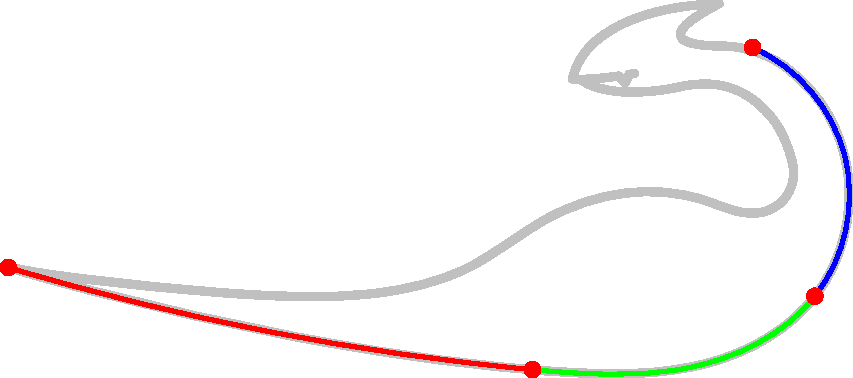
\includegraphics[width=\textwidth]{content/output/examples_spiro_lugia_1.pdf}
							\caption{Lugia \cite{lugia}}
							\label{figure:examples_spiro_lugia_1}
						\end{subfigure}
						\begin{subfigure}[b]{\textwidth}
							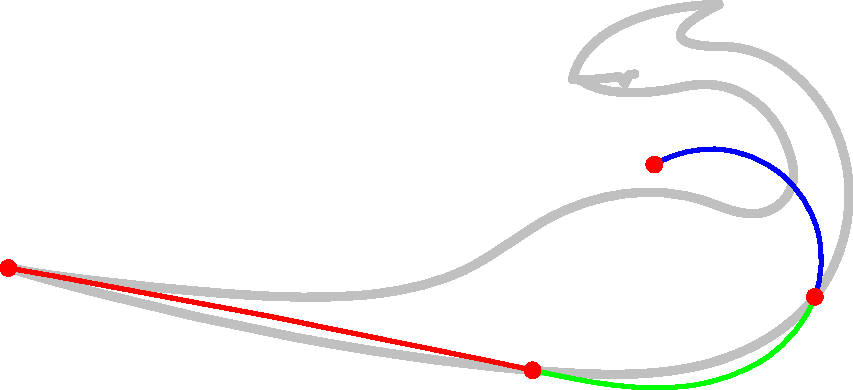
\includegraphics[width=\textwidth]{content/output/examples_spiro_lugia_2.pdf}
							\caption{Lugia \cite{lugia}}
							\label{figure:examples_spiro_lugia_2}
						\end{subfigure}
					\end{minipage}
					\caption{Spiro splines, as they appear in common curve design tools. Control points are displayed as red dots.}
					\label{figure:examples_spiro}
				\end{figure}

				Figure \ref{figure:examples_spiro_fluttershy} shows a shape that is in principle well-suited for being represented by parts of the Euler spiral. Unfortunately, describing the curve using Spiro splines still requires many control points. Note that even though this example has the same number of specified on-curve points (7) as the corresponding example for Bézier splines shown in figure \ref{figure:examples_bézier_fluttershy}, the latter has an additional 12 velocity specifications. This illustrates that even though curvature cannot be specified explicitly, Spiro splines are a much better choice for shapes with approximately linearly changing curvature than Bézier splines.

				Figure \ref{figure:examples_spiro_lugia_1} shows how some shapes can be described using Spiro splines by placing only very few control points. In this case, the shape consists of a circular arc with low curvature (red), a segment of linearly increasing curvature (green) and finally a circular arc with high curvature (blue). This shape can be described conveniently using a Spiro spline with just 4 carefully placed control points.

				Unfortunately, as can be seen in figure \ref{figure:examples_spiro_lugia_2}, this scenario does not handle modifications very well. For instance, increasing the curvature of the blue segment has to be done indirectly by moving a control point, which adversely affects the red segment, since the curvature there was not specified directly but instead relied on the rather fragile configuration of the 4 control points.

	\section{Proposed Solution}
	\label{section:proposed_solution}

		Having analyzed the usability aspect of curve design tools in section \ref{section:problem_analysis}, it is time to think about how to properly address their current issues. In the following sections, we propose both an abstract approach for designing usability-oriented curve design tools, as well as specific ideas for developing software using this approach.
          
		\subsection{Description-Based Curves}
		\label{section:description-based_curves}

			Seeing how the description language almost completely determines all usability aspects of the resulting curve design tool, it seems unwise to base it on low-level mathematical aspects of the curve as is the case with Bézier splines. Spiro splines are much better in that a lot of effort was put into the fairness measure. Unfortunately, the project has set out to solve the problem of constructing interpolating splines, thereby committing to a very restricted specification language right from the start.

			We think that in order to get good usability, using a powerful specification language which does not rely on implementation details has to be the top priority. In combination with a good fairness measure, it forms a description language that, if it allows for reliable and efficient derivation of curves, will then lead to usable curve design tools. Since it is not immediately clear which description language is the best, the first step is to move away from the traditional explicit curve construction, and instead use a process that enables the creation of curves based on descriptions.

			\begin{figure}[htb]
				\centering
				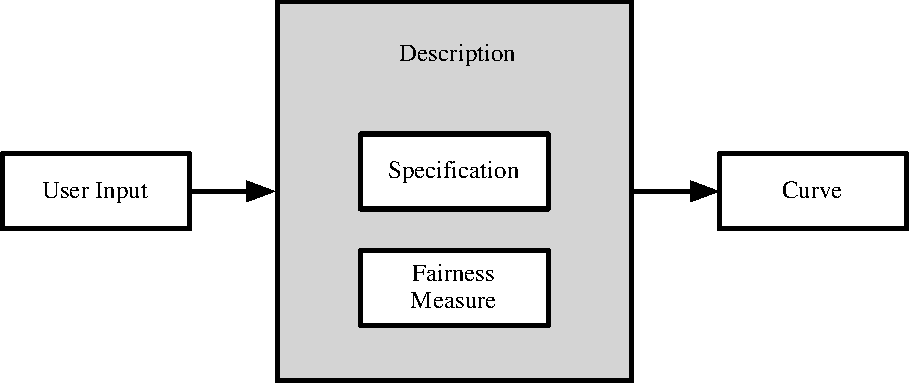
\includegraphics[width=115mm]{content/output/description-based_curves.pdf}
				\caption{Description-Based Curves}
				\label{figure:description-based_curves}
			\end{figure}

			Figure \ref{figure:description-based_curves} shows such a process. Note that this approach does not give any specifics yet, since the previous usability analysis did not give a complete answer as to what the optimal curve design tool looks like. It has yet to be determined what the description language should be, as well as how to derive curves from these descriptions.

		\subsection{Description Language}
		\label{section:description_language}
			
			After establishing the general approach to curve design tools in section \ref{section:description-based_curves}, it is time to decide on the specifics in order to create an instance of this model. The first step is to choose a description language, consisting of both a specification language and a fairness measure.

			The human visual system seems to be fairly insensitive to properties beyond the second derivative of the curve, that is, beyond curvature. Based on that premise, we chose to let the user specify properties up to the second derivative of the curve using the specification language. The fairness measure will then select the curve whose third derivative is minimal from the set of curves that fulfill the specification's requirements.

			\subsubsection{Specification Language}
			\label{section:specification_language}

				The specification language we propose uses differential geometric properties of parametric curves and is thus decoupled from specifics of the underlying curve model, hopefully leading to a specification language that is easier to learn and use. The specification language will focus on the properties point, direction and curvature as defined in section \ref{section:parametric_plane_curves}. In order to provide maximal flexibility, the specification language should allow to specify any combination of these three properties at any number of positions on the curve.

				When only concerned with point specifications, requiring the curve to go through all of them in order may be enough to allow the user to express their intent, although sometimes, even this will lead to undesirable results. That is because even with the curve preserving the order in which the points are visited, it is unspecified how much arc length the curve will spend between each pair of points. When specifying direction and/or curvature without an associated point, it becomes a necessity to associate these specifications with some kind of positional information in order to anchor them to points on the curve. If this were not done, the specifications could move freely along the curve and would therefore behave very unpredictably. We thus chose to associate each combination of point, direction and curvature with a position on the curve.

				With that in mind, it is now possible to abandon this notion of a combination of point, direction and curvature specifications and instead talk about specification items, a specification item being a positioned point-, direction- or curvature specification. For example, a combination of point and curvature specification at some position thus splits up into a point specification item at this position and a curvature specification item at the same position.

				The most simple way of specifying a position on a curve would be by giving a parameter value for the underlying parametric curve. However, this would violate the design idea of using differential geometric properties of curves. A way of specifying a position on a curve that is independent from its parametrization is the arc length of the curve. Instead of directly using the arc length to describe the positions of specification items, we chose to specify positions as fractions of the total arc length of the curve. This way, the position of a specification item relative to the start and end points of the curve is independent of the total arc length of the curve.

				With this setup, it seems advisable to also include the curve's total arc length in the specification. This way, one can sensibly specify curves that have only one point specification item. Also, with unspecified curve length, changing any specification item may inadvertently change the curve's total arc length, thus possibly adversely affecting other parts of the curve whose specification item positions are given as a fraction of the curve's total arc length. For instance, with three point specification items on the curve, pulling the third one further away from the second one would increase the total arc length of the curve. This would also increase the arc length of the curve segment between the first and the second point specification item, thereby unintentionally creating a bulge between those two specification items.

				One way to formally represent the final specification language is as follows:
				\begin{equation*}
					\begin{alignedat}{2}
						& \mathrm{Positions}          && = \unit\\
						& \mathrm{Points}             && = \xc{1} \times \R{2}\\
						& \mathrm{Directions}         && = \xc{2} \times \RR\\
						& \mathrm{Curvatures}         && = \xc{3} \times \RR\\
						& \mathrm{SpecificationItems} && = \mathrm{Positions} \times \left(\mathrm{Points} \cup \mathrm{Directions} \cup \mathrm{Curvatures}\right)\\
						& \mathrm{CurveLengths}       && = \RR\\
						& \mathrm{Specifications}     && = \powerset{\mathrm{SpecificationItems}} \times \mathrm{CurveLengths}
					\end{alignedat}
				\end{equation*}

			\subsubsection{Fairness Measure}
			\label{section:fairness_measure}

				In this section, two important fairness measures are introduced, the minimum energy curve and the minimum variation curve, both of which are characterized by an integral over the arc length of the curve. For the sake of simplicity, the curve will be assumed to have arc length parametrization, such that the integrals are over the curve's parameter on the unit interval.

				Before the advent of computer aided design, mechanical splines made from wood or steel were used in industrial design. People tried to emulate this behavior using mathematical curves, deriving a term for the bending energy in an idealized steel band, which is subsequently minimized. This leads to the following functional describing the minimum energy curve (MEC) \cite{paper-mec}, which tries to minimize the curvature, and thus the bending energy:
				\begin{equation*}
					\integral{0}{1}{\apply{\chi}{t}^2}{t}
				\end{equation*}

				While the minimum energy curve is a good idealization of the mechanical spline, it has some disadvantages when used for curve design. For instance, it will not yield a circular arc when the curve is constrained by co-circular points. Generally speaking, the MEC fairness measure is not very sensitive to bumps and inflection points on the curve, as long as they're small. The human visual system on the other hand, very much is and would always prefer one large arc to multiple small ones. Since the MEC tries to minimize curvature, it is also not suited for the use with curvature specifications, as it will try to bring the curvature back to zero before and after a nonzero curvature specification.

				\begin{figure}[htb]
					\centering
					\begin{subfigure}[b]{\textwidth / 3}
						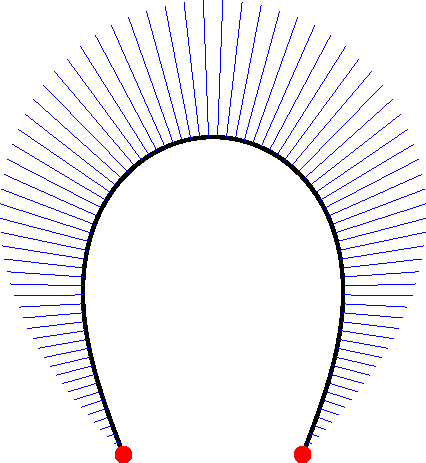
\includegraphics[width=\textwidth]{content/output/fairness_mec_1.pdf}
					\end{subfigure}%
					\begin{subfigure}[b]{\textwidth / 3}
						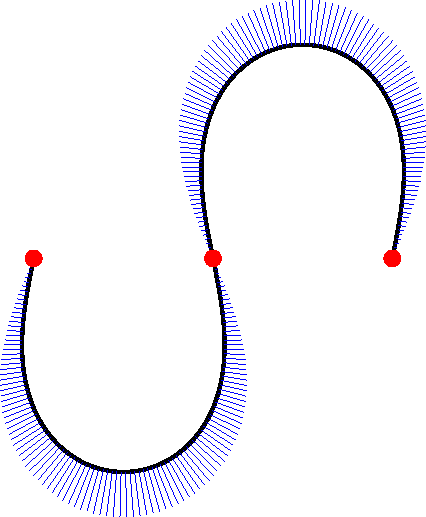
\includegraphics[width=\textwidth]{content/output/fairness_mec_2.pdf}
					\end{subfigure}%
					\begin{subfigure}[b]{\textwidth / 3}
						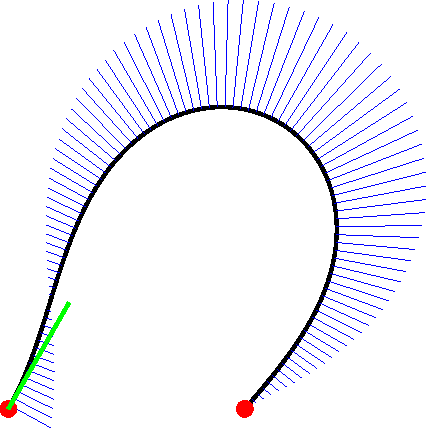
\includegraphics[width=\textwidth]{content/output/fairness_mec_3.pdf}
					\end{subfigure}
					\caption{Examples of minimum energy curves under various constraints. Point specifications are displayed as red dots, direction specifications are displayed as green tangent lines. The thin blue lines visualize the curvature at each point of the curve (longer lines meaning higher curvature).}
					\label{figure:minimum_energy_curve_examples}
				\end{figure}

				Note the characteristic rectangular elastica shapes of the minimum energy curves in figure \ref{figure:minimum_energy_curve_examples}, as well as the fact that, in absence of both direction and curvature specifications, the curvature of a minimum energy curve is always zero at the endpoints.

				In order to address the issues of the MEC, there has been some research into fairness measures whose design is motivated more directly by the human perception of smoothness in plane curves. One such approach is that of the minimum variation curve (MVC) \cite{thesis-mvc}, which tries to minimize the variation of the curvature. The corresponding functional is given below:
				\begin{equation*}
					\integral{0}{1}{\apply{\chi'}{t}^2}{t}
				\end{equation*}

				Minimum variation curves capture the intuitive notion of smoothness very well. The functional will put straight lines through points that are co-linear and circular arcs through points that are co-circular when otherwise unconstrained. When constraints cause different points on the curve to have different curvatures, the fairness measure will prefer linearly changing curvature, as this will result in the derivative of the curvature being constant, thereby minimizing the integral over its square. In general, the MVC fairness measure is very good at avoiding bumps and inflection points when possible. It also works nicely with curvature specifications, since constant curvature is perfectly acceptable for the MVC fairness measure.

				\begin{figure}[htb]
					\centering
					\begin{subfigure}[b]{\textwidth / 3}
						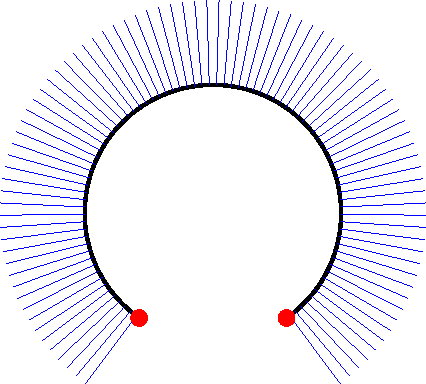
\includegraphics[width=\textwidth]{content/output/fairness_mvc_1.pdf}
					\end{subfigure}%
					\begin{subfigure}[b]{\textwidth / 3}
						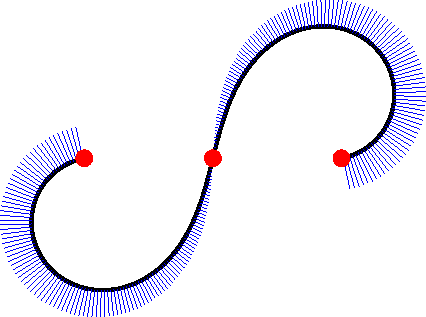
\includegraphics[width=\textwidth]{content/output/fairness_mvc_2.pdf}
					\end{subfigure}%
					\begin{subfigure}[b]{\textwidth / 3}
						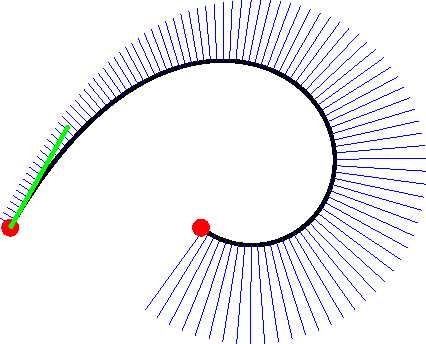
\includegraphics[width=\textwidth]{content/output/fairness_mvc_3.pdf}
					\end{subfigure}
					\caption{Examples of minimum variation curves under the same constraints as the curves in figure \ref{figure:minimum_energy_curve_examples}. Point specifications are displayed as red dots, direction specifications are displayed as green tangent lines. The thin blue lines visualize the curvature at each point of the curve (longer lines meaning higher curvature).}
					\label{figure:minimum_variation_curve_examples}
				\end{figure}

				Note that instead of segments from the rectangular elastica, the characteristic shapes of the minimum variation curves in figure \ref{figure:minimum_variation_curve_examples} are circular arcs and spirals. One may also observe that, instead of trying to bring the curvature to zero towards the endpoints like the MEC does, the MVC tries to establish constant curvature. In contrast to the MEC, the MVC constructs a circular arc in the leftmost example and avoids the inflection point in the rightmost example.

				We think that the minimum variation curve fairness measure is better at producing curves that appear smooth to the human visual system than the minimum energy curve fairness measure. It produces curves that both look good and are close to what the user would expect, given the specification, causing less surprise and frustration when designing curves. Furthermore, it complements the chosen specification language nicely, since, in contrast to the minimum energy curve fairness measure, it works well with curvature specifications. Given these considerations, we have chosen to use the minimum variation curve fairness measure.

		\subsection{Curve Derivation}
		\label{section:curve_derivation}

			Implementing the approach presented in section \ref{section:description-based_curves} requires a way of turning descriptions into actual curves. We chose to use nonlinear optimization on polynomial splines in order to achieve this goal.

			Nonlinear optimization grants some flexibility with respect to the description language, enabling experimentation with different specification languages and fairness measures. This made it possible to assess their usability before settling on the choices presented in section \ref{section:description_language}.

			Polynomial curves were chosen since they are mathematically simple, very flexible through the choice of their degree, and well-suited to approximate a variety of smooth curves. Since polynomials of high degree are known to behave poorly, polynomial splines were used, which allows increasing the segment count, rather than the degree, in order to approximate more complex curves.

			\subsubsection{Optimization Problem}
			\label{section:optimization_problem}

				Nonlinear optimization problems are usually expressed using an objective function \(f : \function{\R{n}}{\RR}\), a constraint function \(g : \function{\R{n}}{\R{m}}\) and constraint bounds \(g_l, g_u \in \R{m}\). The optimization problem is then given by the task of finding an \(x^* \in \R{n}\) such that:
				\begin{equation*}
					\begin{gathered}
						x^* = \argmin_{x \in \R{n}} \apply{f}{x}\\
						g_l \leq \apply{g}{x^*} \leq g_u
					\end{gathered}
				\end{equation*}
				This allows for the expression of a variety of optimization goals, like zero-error constraints (using the constraint function and bounds to specify that an error term should be zero), upper bounds on errors (using the constraint function and bounds to specify an upper bound for an error term) and minimization goals (using the objective function to express that an error term should be minimized).

				The implementation we chose uses smooth optimization, specifically an interior point method. This type of algorithm further requires the functions \(f\) and \(g\) to be at least once, ideally twice continuously differentiable.

				The following sections describe how nonlinear optimization can be used for finding polynomial splines based on descriptions in the language established in section \ref{section:description_language}.

			\subsubsection{Segmentation and Notation}
			\label{section:segmentation_notation}

				The first step is to consider the segment polynomials that make up the polynomial spline used in the optimization. Let \(m\) be the number of segments that make up the polynomial spline and let \(d\) be the degree of each segment polynomial. Then the \(i\)th segment polynomial is given by:
				\begin{equation*}
					\apply{\phi_i}{t} = \sum_{j = 0}^{d} a_{i,j} \cdot t^j
				\end{equation*}
				The functions defined in section \ref{section:parametric_plane_curves} will be used with subscript \(i\) when referring to the \(i\)th segment (\(\apply{\phi_i}{t}\)) and without subscript when referring to the whole spline (\(\apply{\phi}{t}\)). Mapping the parameter \(t\) between the segments and the whole spline works as follows:
				\begin{equation*}
					\apply{\phi}{\frac{i + t}{m}} = \apply{\phi_i}{t}
				\end{equation*}
				That is, the segments are simply laid out consecutively in parameter space, scaled to fit the unit interval, making the parameter mapping function linear and static. Note that these segments are independent of the specification items and are, in fact, completely invisible to the user. Figure \ref{figure:linear_segmentation} shows what the segmentation and parameter mapping look like when using 3 segments.

				\begin{figure}[htb]
					\centering
					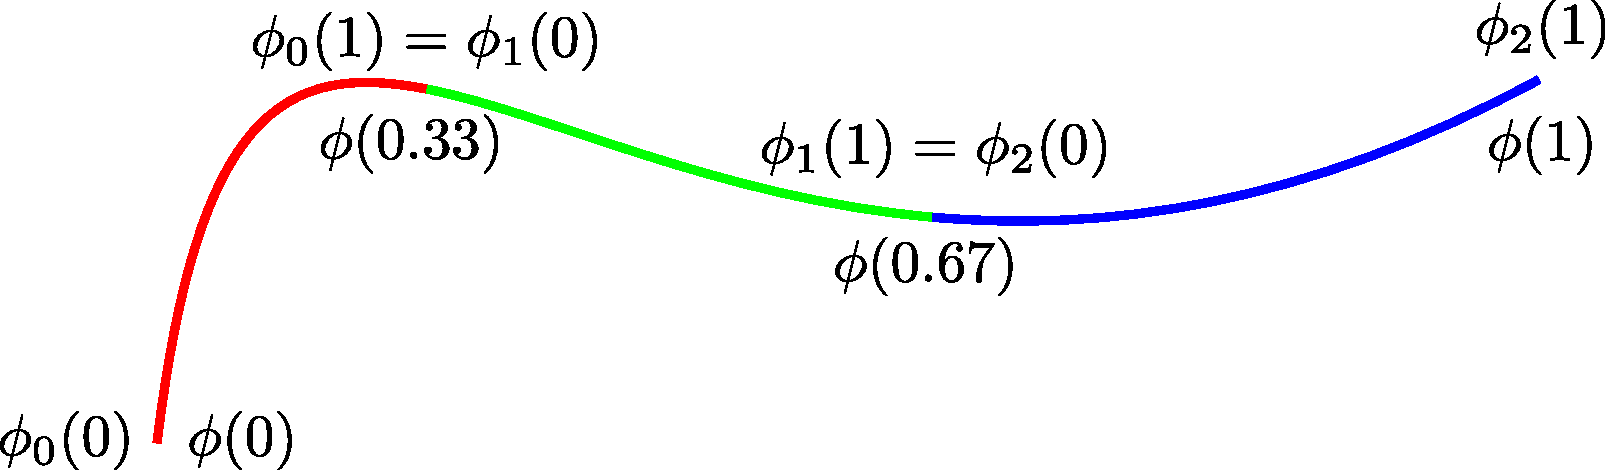
\includegraphics[width=100mm]{content/output/linear_segmentation.pdf}
					\caption{Linear Segmentation}
					\label{figure:linear_segmentation}
				\end{figure}

				Since the polynomial spline is uniquely determined by the coefficients of each segment polynomial, the optimization domain is the vector consisting of all the coefficients \(a_{i,j}\).

				In the following sections, let \(n\) be the number of specification items. Let \(\hat{t}_i\) be the position of the \(i\)th specification item. If the \(i\)th item is a point specification item, the point is denoted \(\hat{\phi}_i\), if it is a direction specification item, the direction is denoted \(\hat{\delta}_i\) and if it is a curvature specification item, the curvature is denoted \(\hat{\chi}_i\). The specified total arc length for the curve is denoted \(\hat{\lambda}\).

			\subsubsection{Constant Speed}
			\label{section:constant_speed}

				As established in section \ref{section:specification_language}, the position of a specification item is given as a fraction of the curve's total arc length, the function mapping the covered arc length to the corresponding parameter values is needed in order to state the optimization goals for the specification items. Unfortunately, this function is not very well-suited to be used as a term in a smooth optimization problem even for simple curves like polynomials. Also, the function is not fixed and varies with the coefficients, so there is no way of telling on which segment each specification item will end up, something else that is difficult to state in a smooth optimization problem. Another problem is that the specification of the total arc length of the curve needs to be stated as an optimization goal, which may be difficult if the the covered arc length function is hard to express. Furthermore, the difficulty of expressing the fairness measure, which is often an integral over the arc length of the curve, is dependent on the complexity of the covered arc length function. In order to address all these problems, the following error term is used:
				\begin{equation*}
					\max_{t \in \unit} \xa{\apply{\sigma}{t} - \hat{\lambda}}
				\end{equation*}
				For polynomial splines with sufficient degree and segment count, this term will be brought close to zero in the optimization, making the speed approximately constant with value \(\hat{\lambda}\). This, in turn, makes the covered arc length function approximately linear (\(\apply{\lambda}{t} \approx \hat{\lambda}t\)), facilitating the simple statement of the optimization goals for the specification items and the fairness measure. It also makes the segment for each specification item fixed. Additionally, it causes the total arc length of the curve to be approximately equal to \(\hat{\lambda}\), as requested by the specification.

				Since this goal can only be fulfilled approximately by polynomial curves, it is impossible to use the error term given above in a zero-error constraint. It could however be used in both an upper bound on errors and in a minimization goal. Both approaches were implemented and tested, with the latter yielding a more stable optimization process.

				The error term given above is not well-suited for smooth optimization because it incorporates finding a maximum. Since the optimization problem will allow the original error term to be brought close to zero, it can be approximated using the following error term:
				\begin{equation*}
					\hat{\lambda}^{-2}\integral{0}{1}{\xp{\apply{\sigma}{t} - \hat{\lambda}}^2}{t}
				\end{equation*}
				As this term is intended to be used as a minimization goal, the factor \(\hat{\lambda}^{-2}\) was added, which makes it scale invariant. This enables the error term to be statically weighted against other terms in the objective function without this weighting being shifted due to curve scaling.

			\subsubsection{Continuity Connections}
			\label{section:continuity_connections}

				As mentioned in section \ref{section:description_language}, we are not concerned with properties beyond the second derivative of the curve. Thus, only \(\contg{2}\) continuity will be required. While the polynomial curves used as segments are smooth (\(\contp{\infty}\) continuity), the resulting spline in general is not. The segments have to be pieced together in such a way as to ensure a certain degree of smoothness. Thus, to ensure \(\contg{2}\) continuity for the whole curve, it is sufficient to ensure \(\contg{2}\) continuity at the segment connection points. To achieve this, the following error terms are added for each connection point (\(0 \leq i \leq m - 1\)):
				\begin{equation*}
					\begin{gathered}
						\apply{\phi_i}{1} - \apply{\phi_{i + 1}}{0}\\
						\apply{\phi'_i}{1} - \apply{\phi'_{i + 1}}{0}\\
						\apply{\phi''_i}{1} - \apply{\phi''_{i + 1}}{0}
					\end{gathered}
				\end{equation*}
				These error terms being zero implies \(\contp{2}\) continuity. However, since the constant speed requirement introduced in the previous paragraph collapses \(\contp{2}\) continuity and \(\contg{2}\) continuity, this is equivalent to the original requirement of ensuring only \(\contg{2}\) continuity, yet better suited for optimization. 

				It is not acceptable for the curve segments to not touch, have sharp corners or curvature discontinuities, so the error terms above are added as zero-error constraints.

			\subsubsection{Specification Items}
			\label{section:specification_items}

				With the technical details arising from the use of polynomial splines taken care of, the error terms for the specification items can be stated. Since the optimization goal in section \ref{section:constant_speed} ensures that \(\apply{\lambda}{t} \approx \hat{\lambda}t\), the whole spline is parametrized such that the parameter \(t\) is a fraction of the curve's total arc length. This fits perfectly with the fact that the position of each specification item is also specified as a fraction of the curve's total arc length. Thus, for each specification item (\(0 \leq i \leq n\)), one of the following error terms is added, depending on the type of the specification item:
				\begin{equation*}
					\begin{gathered}
						\apply{\phi}{\hat{t}_i} - \hat{\phi}_i\\
						\apply{\delta}{\hat{t}_i} - \hat{\delta}_i\\
						\apply{\chi}{\hat{t}_i} - \hat{\chi}_i
					\end{gathered}
				\end{equation*}

				The user usually wants to specify exact curve behavior rather than indirectly influencing properties, so these error terms are added as zero-error constraints.

			\subsubsection{Fairness Error}
			\label{section:fairness_error}

				After establishing constant speed in section \ref{section:constant_speed}, the error term for the fairness chosen in section \ref{section:fairness_measure} is well-suited for smooth optimization:
				\begin{equation*}
					\hat{\lambda}^2\integral{0}{1}{\apply{\chi'}{t}^2}{t}
				\end{equation*}
				Whenever there is non-constant curvature, this error term will not be zero, and in fact, may be arbitrarily large. Thus, it is not suitable to be constrained to zero or be used as a bounded error and has to be stated as a minimization goal. Note that similar to the error term for constant speed, the factor \(\hat{\lambda}^2\) is added, which causes the fairness measure to be invariant under scaling of the whole curve. This enables static weighting of error terms in the objective function.

			\subsubsection{Final Assembly}
			\label{section:final_assembly}

				Having gathered all the necessary error terms, they are assembled in a nonlinear optimization problem. Terms with zero-error constraints, as well as terms with upper bounds on the error are added as component functions of the constraint function \(g\) together with appropriate bound components in \(g_l\) and \(g_u\).

				Minimization goals, on the other hand, are assembled in a weighted sum which defines the objective function \(f\). Since the error terms were designed to be scale invariant, this weighting can be done statically. The exact values of the weights are to be determined empirically.

				Once the optimization problem is put together, it is passed to the optimization solver, which will return the optimized coefficients of the segment polynomials. These segment polynomials are then assembled according to the layout described in section \ref{section:segmentation_notation} in order to obtain the final curve.

	\section{Implementation}
	
		In this section, the implementation of our prototype, referred to as Kurve in short, will be described.

		\subsection{Architecture}
			
			\subsubsection{Programming Language}
			
				The first step of the implementation of the proposed solution is the choice of the platform and development environment that will be used. 
				As the programming language, C\# is the best option due to the following features:
				
				\begin{itemize}
				  	\item Platform independence - the project is not bound to any specific platform and can be used on all major operating systems, provided the libraries Kurve depends on are available. 
				  	\item C\# is a high-level language - this reduces overhead in the development process, for example spending time on manual memory management.
					\item Ability to interface with native code - native code can be interfaced with by using reasonable amounts of boilerplate code. Native libraries are used in Kurve, therefore this is a key requirement.
					\item Familiarity - the developers are familiar with this language. This choice eliminates overhead that would be caused by adopting an unfamiliar language.
					\item UI frameworks - part of the project is a proof of concept user interface to work with curves. Several UI frameworks are available that interface directly with C\#.
				\end{itemize}
			
			\subsubsection{Libraries}
				
				Kurve offers its own APIs in C\# for working with terms and optimization problems. However, the implementation of the functionality of these APIs is provided by third-party libraries. Hence, Kurve relies on several libraries, including:
				
				\begin{itemize}
				  	\item Ipopt\footnote{https://projects.coin-or.org/Ipopt} is a library that does numeric non-linear optimization. It allows to solve optimization problems as described in \ref{section:optimization_problem}.
					\item CasADi\footnote{http://casadi.org} provides functionality to perform automatic differentiation of terms. It interfaces with Ipopt directly, which makes it the preferred choice for the symbolic differentiation required in Kurve. CasADi is written in C++, but unfortunately only C functions can be called easily from C\#. For that reason, a small CasADi wrapper written in C was required to implement Kurve's C\# term APIs. 
				\end{itemize}
			
				 Kurve has strong requirements for both libraries: Terms used in the functions that need to be optimized in Kurve are large and plentiful, but differentiation and optimization still need to be performed in a short period of time to allow real-time editing of curves. Fortunately, CasADi and Ipopt are very efficient and allow Kurve to offer close to real time editing of curves.

				For Kurve's user interface, GTK\#\footnote{http://www.mono-project.com/GtkSharp} was used. GTK\# provides functionality to draw the curves and controls into a window, as well as handling keyboard and mouse events.
				
			\subsubsection{Subsystem Decomposition}	
			
				\begin{figure}[htb]
					\centering
					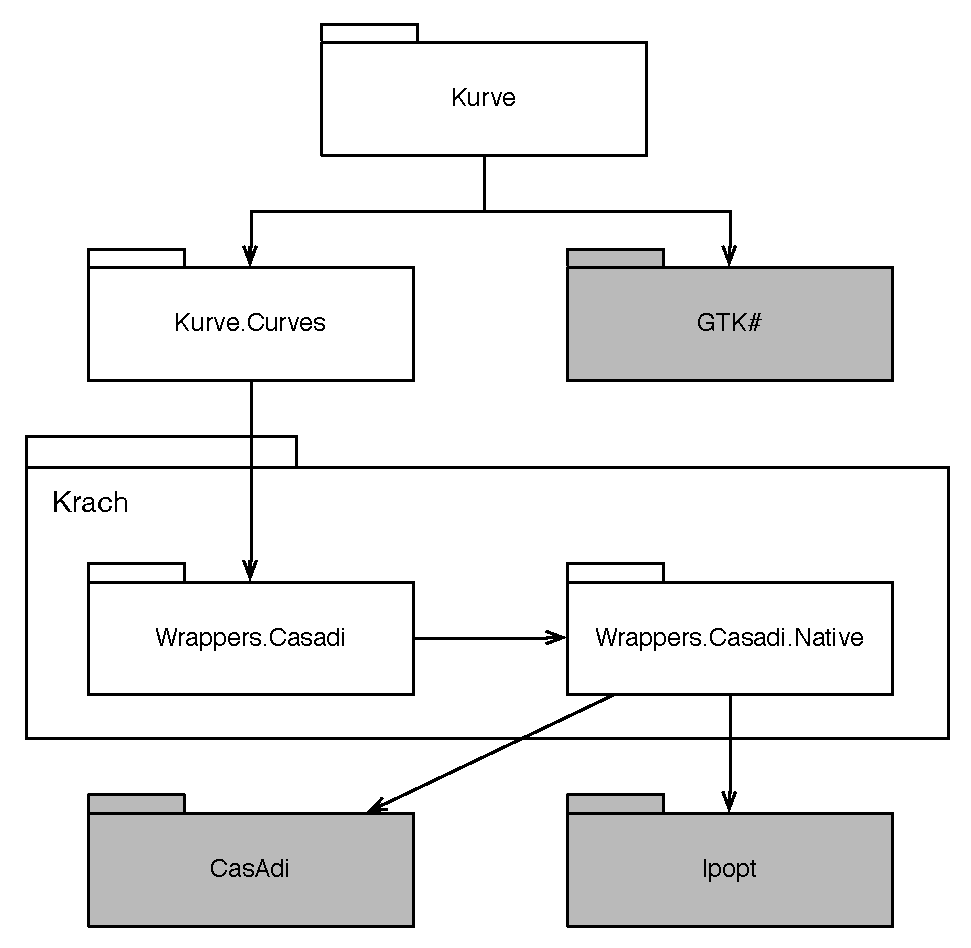
\includegraphics[width=110mm]{content/output/subsystems.pdf}
					\caption{Subsystem Decomposition of the Kurve Project}
					\label{figure:subsystem_decomposition}
				\end{figure}
				
				Kurve's implementation is split into two primary subsystems: \verb|Kurve| contains the user interface related code and has a dependency on GTK\# as well as \verb|Kurve.Curves|; \verb|Kurve.Curves| is responsible for generating curves from specifications using CasADi through \verb|Wrappers.Casadi|. 
				
				 \verb|Wrappers.Casadi| and \verb|Wrappers.Casadi.Native| contain a wrapper for CasADi using C\# and C++ code respectively. \verb|Wrappers.Casadi| relies on \verb|Wrappers.Casadi.Native|. 
				 
				 \verb|Wrappers.Casadi| and \verb|Wrappers.Casadi.Native| are now part of the general-purpose library Krach to allow easy reuse in other projects.
		
			\subsection{Numerical Optimization}
				The \verb|Kurve.Curves| project contains the code required to transform input specifications into curves. It relies on CasADi (through \verb|Krach.Wrappers.Casadi|) to represent curves symbolically and on Ipopt for optimization.
			
				\subsubsection{Specification}
					\begin{figure}[htb]
						\centering
						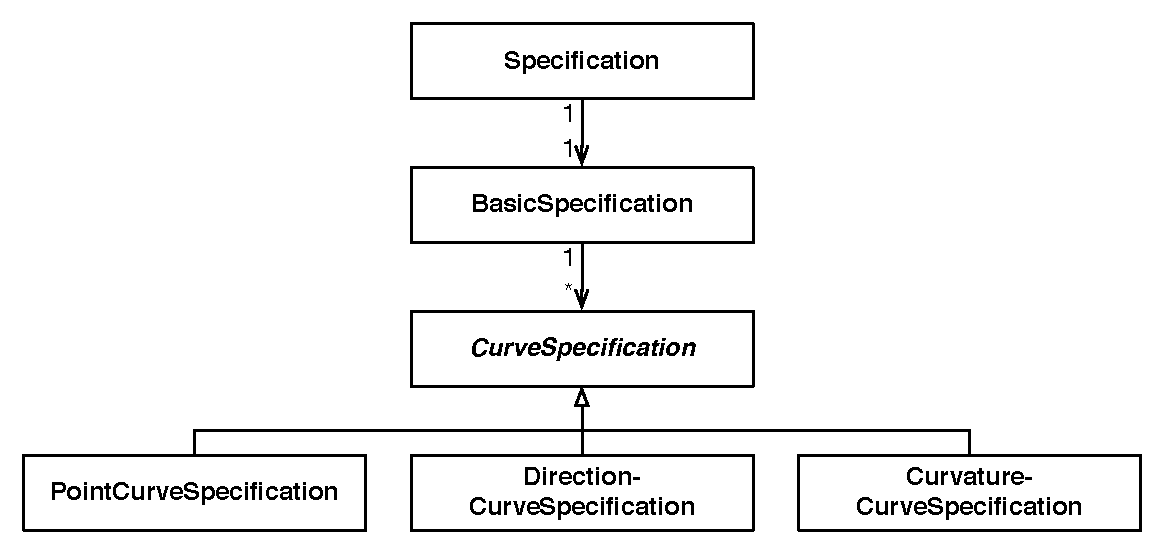
\includegraphics[width=135mm]{content/output/specification_class_diagram.pdf}
						\caption{Class Diagram of Specification-Related Classes}
						\label{figure:specification_class_diagram}
					\end{figure}
				
					To fully specify a curve, several different pieces of information are needed:
				
					\begin{itemize}
						\item Any number of point, direction and curvature specifications. These \verb|CurveSpecification|s are stored in a \verb|BasicSpecification|.
						\item The curve's total length is also part of a \verb|BasicSpecification|.
						\item The curves are represented using a number of segments, each of which is represented by some function, realized using the \verb|FunctionTermCurve| class. Because of that, the number of segments as well as the function type that is used to represent each segment are part of \verb|BasicSpecification| as well. 
						The type of function used is represented using a \verb|FunctionTermCurveTemplate| object. This template allows the creation of \verb|FunctionTermCurve| objects.  
						However, this information is only used during optimization. If the number of segments and function template yield a curve with enough degrees of freedom with respect to the other specifications, roughly the same curve will be generated even if the number of segments and function template is changed. It is possible to specify the segment count and function template to modify the degrees of freedom that the resulting curves offers (i.e. more degrees of freedom mean the curve can satisfy more curve specifications while maintaining constant speed and good fairness, but the optimization process takes longer).
						\item Curves could be generated from a \verb|BasicSpecification| alone. However, if there are multiple curves that fit a \verb|BasicSpecification| very well (i.e. the optimization problem has multiple local optima), different actual curves could be generated from a \verb|BasicSpecification|. One problem that can arise when saving a curve, if only the \verb|BasicSpecification| were saved, it would be possible that a different curve is displayed when loading the curve, because a different local optimum was reached in the optimization process. This is undesirable and a way to disambiguate between the different optima is required. 
						For that reason, a full \verb|Specification| consists of a \verb|BasicSpecification| as well as some disambiguation information. That disambiguation information is the result of the optimization, which can be used as a starting position for the optimization process when a curve is loaded. This ensures that the same curve will be generated and speeds up the optimization process as well.
					\end{itemize}
				
				
				\subsubsection{Optimization}
					\begin{figure}[htb]
						\centering
						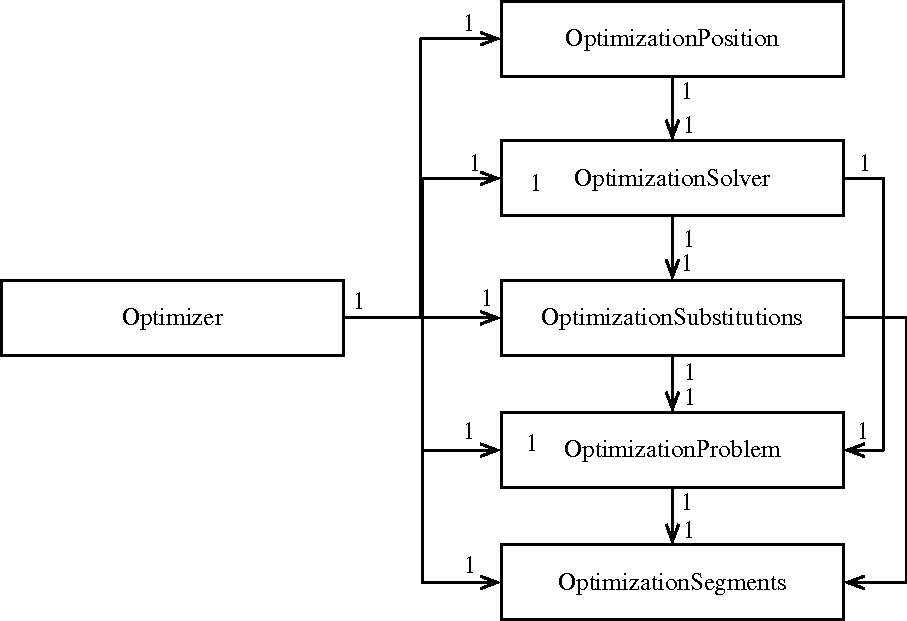
\includegraphics[width=110mm]{content/output/optimization_class_diagram.pdf}
						\caption{Class Diagram of Optimization-Related Classes}
						\label{figure:optimization_class_diagram}
					\end{figure}
					
					The \verb|Optimizer| class handles the optimization process of a curve. By supplying a \verb|Specification|, a concrete curve as well as a new \verb|Specification| with updated disambiguation information can be obtained. The resulting curve is represented by a \verb|Curve| object which allows access to the curve's points, speed, direction and curvature, but carries no information about the internal segmentation and function type used.
					
					The optimization process is performed in a number of steps. Depending on the change of the specification, only certain steps have to be run again as previous results can be reused.
					
					\begin{description}
						\item[Segments]
						In the first step curve segments are created based on the number of segments and the segment template specified in the \verb|BasicSpecification|. A list of parameters of all segments is created. By applying concrete values to each of the parameters, a curve can be obtained. The generated segments are cached and do not have to be regenerated if the number of segments and segment template specified in the \verb|BasicSpecification| do not change.
						
						\item[Optimization Problem]
						Next, the optimization problem is created. The optimization problem specifies an objective function which includes the speed error discussed in section \ref{section:constant_speed} as well as the fairness function discussed in section \ref{section:fairness_error}. Furthermore the continuity connections discussed in section \ref{section:continuity_connections} and the satisfaction of the curve's specificationsare realized using a constraint function. This step also computes the first and second derivatives of those functions. The concrete values required by the curve specifications are not used. Instead, placeholder variables are introduced. For the total length of the curve a placeholder is used as well. This allows the reuse of the optimization problem if curve specifications or curve length change. The derivatives do not have to be recomputed. Thus, the optimization problem is cached and only rebuilt if the optimization segments change or if the number of each type of constraint on the curve changes. If the value of a constraint changes, but the type of constraint remains the same (e.g. a point constraint requires the curve to pass through a different point than before), the optimization problem does not have to be rebuilt.
						
						\item[Substitutions]
						In this step, substitutions for each of the placeholder variables (i.e. for each curve specification and the curve length) are created. These substitutions, when applied to an optimization problem, remove all placeholder variables and yield the optimization problem that needs to be solved to obtain a concrete curve. The substitutions have to be rebuilt whenever a specification changes, the total curve length changes, or any of the previous steps had to be recomputed.
						
						\item[Solver]
						In this step, a solver for the optimization problem is created. The solver used is provided by Ipopt. A new solver needs to be created whenever either the optimization problem or the substitutions change.
						\item[Position]
							The position represents a result of an optimization process. To obtain this, the solver created in the previous step is run. As the starting position, the previous optimization's position is used. Using the obtained position, a concrete curve can be obtained from the optimization segments. This curve is the desired end result returned by the Optimizer.
					\end{description}
					
					
			\subsection{User Interface Implementation}
				\begin{figure}[htb]
					\centering
					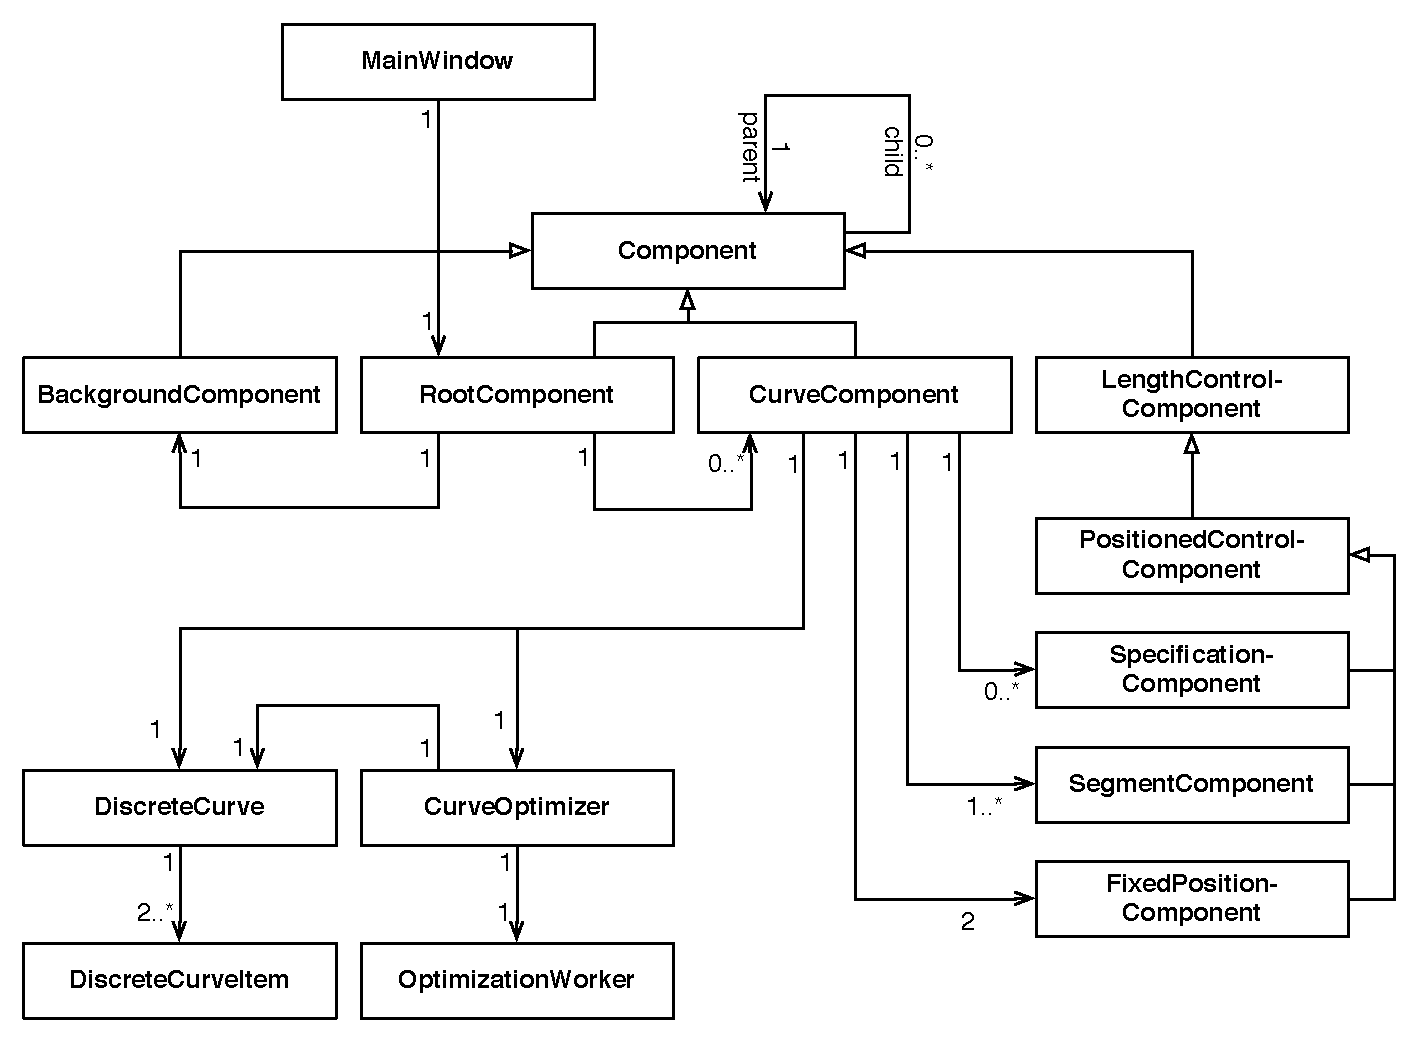
\includegraphics[width=\textwidth]{content/output/ui_components_class_diagram.pdf}
					\caption{Class Diagram of the User Interface Components}
					\label{figure:ui_components_class_diagram}
				\end{figure}
				
				Kurve's user interface is constructed from \verb|Component|s. \verb|Component|s may contain a number of subcomponents, render themselves into a GTK\# context, and handle mouse and keyboards events. 
				\begin{itemize} 
					\item \verb|MainWindow| - The \verb|MainWindow| is a GTK\# window that contains the \verb|RootComponent|. It triggers redraws of the \verb|RootComponent| when appropriate (e.g. when the window is resized) and forwards mouse and keyboard events to the \verb|RootComponent|.
					\item \verb|Component| - \verb|Component| is the abstract base class of all components that make up Kurve's user interface. It provides default implementations for rendering components, handling mouse and keyboard events, and provides a mechanism to trigger redraws of subcomponents.
					\item \verb|RootComponent| - The \verb|RootComponent| manages a list of \verb|CurveComponent|s and implements functionality to add and remove curve components. Additionally, the \verb|RootComponent| implements save and load functionality.
					\item \verb|BackgroundComponent| - This component can display a background image. This can be used to trace existing images with the Kurve tools.
					\item \verb|CurveComponent| - This component represents a curve in the user interface. It consists of several \verb|PositionedControlComponent|s (any number of \verb|SpecificationComponent|s and a \verb|FixedPositionComponent| at both the start and the end of the curve). This yields segments of the curve - one segment between each pair of \verb|PositionedControlComponent|s. These segments are represented by \verb|SegmentComponent|s. A \verb|CurveOptimizer| is used to create a curve from the specifications given by the \verb|SpecificationComponent|s. \verb|CurveComponent| implements functionality to add and remove \verb|SpecificationComponent|s and to change the curve template used (e.g. change the degree of the polynomial template). 
					\item \verb|LengthControlComponent| - A \verb|LengthControlComponent| is a \verb|Component| that can modify the length of the \verb|Curve| in a certain area.
					\item \verb|PositionedControlComponent| - A \verb|PositionedControlComponent| is a component that has a specific position on the curve. 
					\item \verb|SpecificationComponent| - A \verb|SpecificationComponent| allows to specify constraints on a curve. A point, direction and/or curvature can be specified for a given position using various mouse and keyboard commands. \verb|SpecificationComponent|s are visualized as a small black box that can be selected.
					\item \verb|FixedPositionComponent| - \verb|FixedPositionComponent|s represent the start and end of a \verb|CurveComponent|.
					\item \verb|SegmentComponent| - A \verb|SegmentComponent| represents a section of a curve delimited by two \verb|PositionedControlComponents|. The \verb|SegmentComponent| renders the curve in that segment, but it also allows to modify the length of the curve in that segment.
					\item \verb|DiscreteCurve| and \verb|DiscreteCurveItem| - A \verb|DiscreteCurve| represents the data necessary to render a curve in the user interface. It contains information about the curve's points, direction, and curvature. It is represented by a number of \verb|DiscreteCurveItem|s that sample a source curve's point, direction and curvature at certain positions. 
					The \verb|CurveOptimizer| yields this type of curve. The reason why this kind of discrete curve is used is due to the lack of the ability to use \verb|Curve| and \verb|Optimizer| (from the \verb|Kurve.Curves| subsystem) at the same time. This, in turn, is caused by the CasADi library, which is not thread safe. However, CasADi is used for representing \verb|Curve|s internally, as well as for performing optimization tasks.
					As Kurve uses a background thread to optimize curves, it is not possible to use the \verb|Curve| objects yielded by the optimizer to render the curves in the main thread at the same time. For that reason, \verb|Curve| objects are converted to \verb|DiscreteCurve| objects in that background process.
					\item \verb|CurveOptimizer| and \verb|OptimizationWorker| - The optimization process required to generate a curve from specifications takes too much time to perform in the main thread (the user interface would be blocked for too long), therefore optimization is performed in a background thread. Each \verb|CurveComponent| uses a \verb|CurveOptimizer| to submit changed specifications. A single shared \verb|OptimizationWorker| handles the synchronization and makes sure each submitted specification gets processed one by one. It is necessary to ensure that no optimization processes run in parallel, as the CasADi library (which is used in this process) is not thread safe.
				\end{itemize}

			\subsection{Using Kurve}
				
				The user interface does not focus on user friendliness. Its purpose is to test the validity of the approach to curve design researched in this project. For that reason, most actions are performed using keyboard shortcuts. Many user interface elements can be selected with the mouse. This enables to use keyboard shortcuts that affect that component only. It is possible to interact with some components using the mouse. However, there is no toolbar or similar user interface elements that would make any of the features more accessible.
				
				The user interface allows the user to:
				\begin{itemize}
					\item add curves
					\item add specification controls to curves (specifying point, direction and/or curvature at a certain position on the curve) 
					\item control the curve's length (using specification and segment controls)
					\item control the degree of the polynomial template and the number of internal segments of the curve
					\item display a background image (e.g. to trace curves in an existing image)
					\item save and load curves
				\end{itemize}
				
				\begin{figure}[htb]
					\centering
					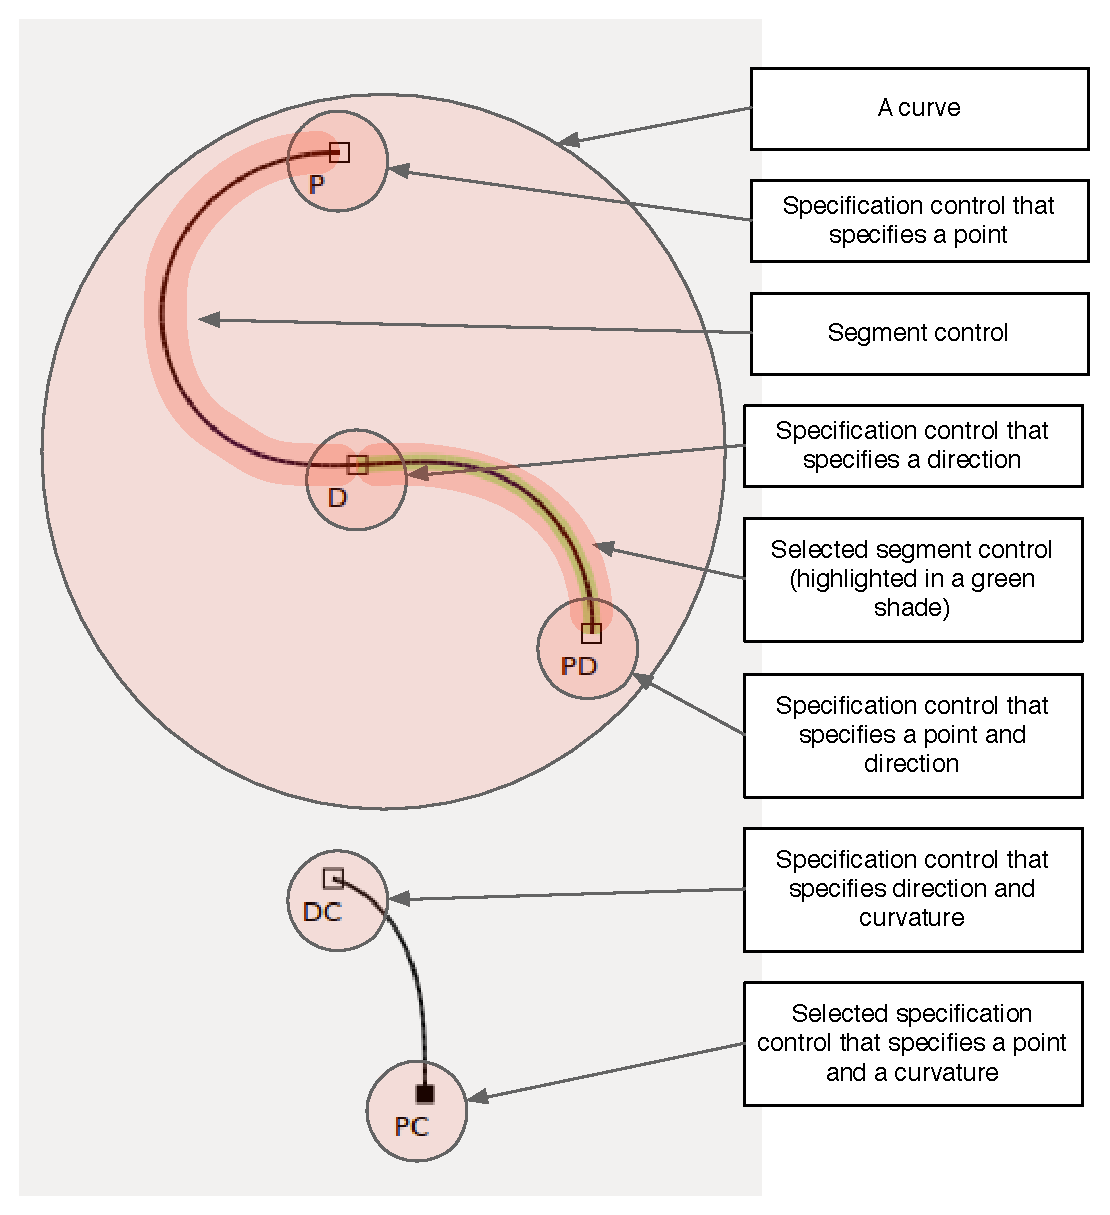
\includegraphics[width=130mm]{content/output/ui_components.pdf}
					\caption{Overview of the User Interface in Kurve}
					\label{figure:ui_components}
				\end{figure}
				
				\subsubsection{General Commands}
				
					A curve can be added by pressing `N'. A new curve will appear in window that is initialized with a length of 100, and two specification controls specifying points. The curve uses one segment that uses a polynomial curve template with a degree of 10.
					
					To save all curves in the window, press `S'. A save file dialog will appear that allows the user to specify a file name. Saved files can later be loaded by pressing `L' which displays an open file dialog. Keep in mind that loading a file dismisses all curves in the current window.
					
					A background image can be displayed by passing a path to an image file when launching the Kurve application.
					
				\subsubsection{Curves}
					
					Click the right mouse button anywhere on a curve to add a specification control at that position. The newly added specification control does not yet specify anything. To remove a specification control, select it and press `R'. See the section \ref{section:specification_control} on how to use specification controls. 
					
					The length of the curve can be modified by selecting specification controls and segment controls and using the mouse wheel while pressing shift. If a specification control is selected, length is inserted to the left and right of the specification control; if a segment control is selected, that segment's length is changed.
					
					The current version of Kurve uses polynomial functions in each segment. The template that generates the functions and the number of segments can be modified as follows:
					
					\begin{itemize}
						\item To change the number of segments used, press `1' to decrease and `2' to increase the number of segments by one.
						\item To change the degree of the polynomial used in each segment, press alt + `1' to decrease, and alt + `2' to increase the degree by one.
					\end{itemize}
					Keep in mind that the segment count and the degree of the polynomials are not directly visible to the user and are used in the optimization process only. Adding more segments or increasing the degree of the polynomials allows more complicated curves, but has negative effects on the performance.
				\subsubsection{Specification Control}
				\label{section:specification_control}
				
					A specification control on a curve can specify any combination of a point, direction, or curvature at a certain position on the curve. Any combination of the three following letters represent which geometric attributes are specified by the specification control. 
					
					\begin{itemize}
						\item `P' indicates that a point that the curve has to pass through at that position is specified.
						\item `D' indicates that the direction of the curve at that position is specified.
						\item `C' indicates that the curvature of the curve at that position is specified.
					\end{itemize}
					
					Which attributes are specified can be toggled by selecting a specification component by clicking it and pressing the corresponding key on the keyboard. Which attributes are currently being specified is displayed in a label below the specification control. For example, if the label shows `n/a', nothing is specified, while `PC' indicates that a point and a curvature are specified.
					
					When a geometric attribute is specified by a specification control, it can be modified:
					
					\begin{itemize}
						\item Point: The point can be modified by dragging the specification control with the mouse.
						\item Direction: The direction can be modified using the mouse wheel.
						\item Curvature: The curvature can be modified by pressing the windows key while using the mouse wheel.
					\end{itemize}
					
					The position of the control can be modified by pressing the control key while using the mouse wheel. Keep in mind that when changing the position of a specification control that does not specify a point, the control itself will most likely move (and change its point).
					
					To achieve more fine-grained control, it is possible to press the alt key while performing any of the actions described above. This changes the affected property of the specification control more slowly. For example, if you press alt while dragging a specification control, it will move very slowly.
					
					As an experimental feature, it is also possible to change the position of a specification control by dragging it with the mouse while pressing shift. The position is calculated by the current state of the curve.
				
				\subsubsection{Segment Control}
				
					A segment control is a part of a curve delimited by either two specification controls or the start/end of the curve. It can be selected by clicking it.
					
					If at least one of the delimiting controls specifies a point, segments can be moved by dragging them with the mouse.
					
					A segment also displays the speed of the curve if it differs from the optimal speed. Too high speed is indicated by a red hue. This can usually be fixed by inserting additional length. Too low speed is indicated by a blue hue. Usually there will be both blue and red sections. This may indicate that the curve is too complex (i.e. there are too many specifications) to achieve a good representation with the current curve template. This can be fixed by either removing specifications, adding internal segments to the curve, or increasing the degree of the polynomial function template used in the curve.
				
				\begin{figure}[htb]
					\centering
					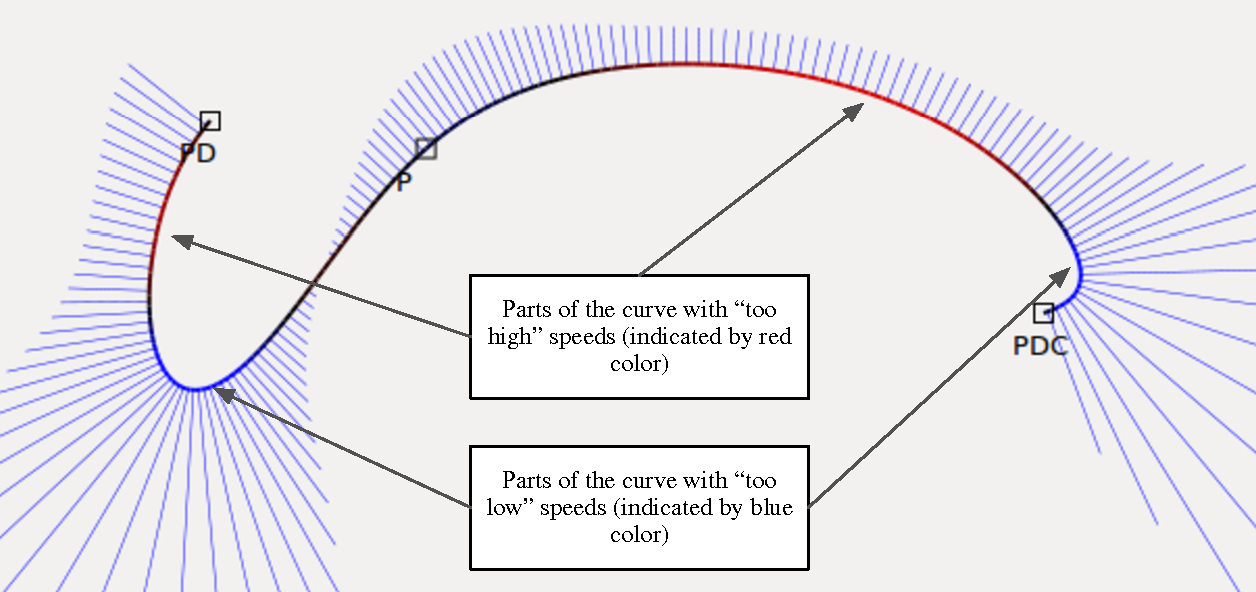
\includegraphics[width=\textwidth]{content/output/ui_speeds.pdf}
					\caption{Example of a Curve that is `overspecified' (i.e. the speed of the curve cannot be kept constant due to the high amount of constraints)}
					\label{figure:ui_speeds}
				\end{figure}
				
				\subsubsection{Command Cheat Sheet}
					\begin{itemize}
						\item General
						\begin{description}
							\item[`N'] Add a new curve
							\item[`L'/`S'] Load/Save
							\item[`1'/`2'] decrease/increase internal segment count
							\item[Alt + `1'/`2'] decrease/increase polynomial template degree
						\end{description}
						\item All Controls
						\begin{description}
							\item[Click] Selects a control 
							\item[Shift + Click] Select multiple controls
							\item[Shift + Scroll (+ Alt)] Insert length at component (slowly)
						\end{description}
						\item Specification Control
						\begin{description}
							\item[Ctrl + Scroll (+ Alt)] Change the position of the specification (slowly)
							\item[Shift + Drag] Change position of specification (adjusts the point of the specification)
							\item[`R'] Removes the specification
							\item[`P'] Triggers point specification
							\item[Drag (+ Alt)] Move point (slowly). Only possible when point specification is enabled.
							\item[`D'] Triggers direction specification
							\item[Scroll (+ Alt)] Changes the direction (slowly). Only possible when direction specification is enabled.
							\item[`C'] Triggers curvature specification
							\item[Win + Scroll (+ Alt)] Changes the curvature (slowly). Only possible when curvature specification is enabled.
							\item[Shift + Click] Select multiple controls
							\item[Shift + Scroll (+ Alt)] Insert length at component (slowly)
						\end{description}
						\item Segment Control
						\begin{description}
							\item[Right-Click] Add empty specification control at that position
							\item[Drag] Moves any point specifications delimiting the segment. (Only possible if at least one of the specification controls has the point specification enabled.)
						\end{description}
					\end{itemize}
		
	\section{Evaluation}
	\label{section:evaluation}

		The goal of this project was to explore possible improvements concerning the usability of curve design tools. The following sections discuss the results in this area.

		\subsection{Usability Analysis}
		\label{section:usability_analysis}

			Having applied the usability criteria from section \ref{section:usability_criteria_curve_design_tools} to Bézier splines and Spiro splines, they are finally used to evaluate the usability aspects of the prototype curve design tool.

			\subsubsection{Expressiveness of the Description Language}
			\label{section:expressiveness_description_language}

				One of the primary goals of this project was to explore more expressive description languages than those which are currently used in vector graphics software. To that end, the chosen specification language supports specifying points, directions and curvatures at any number of positions on the curve, as well as the total length of the curve. Furthermore, the fairness measure ensures constant and linearly changing curvature where possible. This grants the user much flexibility in describing the source curve, allowing them to specify those properties which can describe the curve in the most concise fashion.

				The ability to specify curvature constitutes a significant improvement over common curve design tools, where this is usually not possible. Using this functionality, the user can specify curves which are best expressed in terms of curvature in a natural and concise way. Not only does this make the curve design process less tedious, but it may also lead to better curves, since only the essential information about the curve is provided to the software. This allows the fairness measure to choose the best curve, something that is not possible if lots of information is supplied to the software in order to indirectly influence the curvature.

				Curvature specifications are especially useful in conjunction with the MVC fairness measure, which selects constant or linearly changing curvature where possible. This way, placing curvature specifications on an otherwise unconstrained curve allows the user to precisely create spirals. This behavior of the fairness measure also makes it possible to construct circular arcs in various ways, since they are the preferred shape of curve.

				Section \ref{section:specification_language} describes why it makes sense to force the specification of the curve's total arc length. Fixing the arc length of the curve (and thus also the arc length between each specification item) may seem a little restrictive at first, however, there are actually quite a few upsides. For instance, by adjusting the arc length of a curve with a point specification item on each end, one can conveniently produce circular arcs between two points. This is because increasing the arc length will make the curve bulge out, with the fairness making sure that a circular arc is produced. Generally speaking, having control over the arc length of the curve results in benign and predictable curve behavior and is often useful for pulling it in place, not unlike the way one would handle a mechanical spline.

				On the other hand though, it is not possible not to specify the curve's arc length, and there may be cases where the user wants to leave it to the fairness measure to choose the best arc length for the curve. While it is sometimes possible to work around this issue by placing direction and/or curvature specification items instead of point specification items, that may not always be the case. Further investigation into how arc length specification can be made optional while avoiding the problems mentioned in section \ref{section:specification_language} is necessary.

				As a final way of demonstrating the high expressiveness of the description language, it may be noted that it actually allows for the description of arbitrary segments of the Euler spiral. Since every segment of the Euler spiral exhibits linearly changing curvature between its start and end points, specifying these curvature values on an otherwise unconstrained curve will cause the fairness measure to select the desired segment of the Euler spiral.

			\subsubsection{Human Interaction with the Specification Language}
			\label{section:human_interaction_specification_language}

				The specification language is based on the familiar differential geometric properties point, direction, curvature and arc length, all of which have a simple geometric interpretation and are thus easy to understand.

				Points, directions and curvatures are easy to extract from a given source curve. While extracting the arc length of a long curve may be difficult in some cases, this is usually not required since the arc length is mostly adjusted locally, where it is fairly easy to estimate.

				Since curves can usually be described using only a few specification items, communicating this information to the curve design tool is not too difficult either. Points are well-suited to be specified using the mouse pointer. The current prototype curve design tool only supports very basic input facilities for direction and curvature, resulting in some difficulties when creating and modifying these specification items. This could easily be fixed by utilizing their geometric interpretation, letting the user specify tangent lines and osculating circles instead of raw numeric values. Arc lengths are usually specified locally and by repeatedly making small adjustments, making them relatively easy to handle.

			\subsubsection{Smoothness and Minimality of Curves Selected by the Fairness Measure}
			\label{section:smoothness_minimality_curves_selected_fairness_measure}

				As described in section \ref{section:fairness_measure}, the MVC fairness measure captures the intuitive notion of smoothness very well, resulting in aesthetically pleasing curves.

				Unfortunately, the nonlinear optimization approach to finding the best curve can only find local optima, such that in many cases, the curve is not minimal, often containing loops and unnecessary inflection points. However, this is usually easy to fix by adjusting the specification in such a way that the global optimum is found. For instance, a loop in the curve can often be removed by placing an additional point specification item on the loop, pulling it away from the curve until it is forced to straighten out and finally removing the point specification item again. Once the curve has been pushed into the global optimum like this, it is usually very stable.

			\subsubsection{Ability to Derive Curves from Descriptions}
			\label{section:ability_derive_curves_descriptions}

				As mentioned in section \ref{section:curve_derivation}, using nonlinear optimization has many advantages for research and proof of concept projects like this one. Unfortunately, the flexibility it grants comes with a price, in that it is much slower and also less reliable than unique mathematical constructions like the ones used for Bézier splines.

				Even on very powerful computers, running nonlinear optimization on splines with many segments and/or polynomials of high degree is too slow for interactive curve design, with updates taking seconds. Most curves are very simple and do not need this kind of complexity, but for those that do, the bad performance can be very disruptive.

				Another issue is reliability. For some descriptions, the iterative optimization algorithm may converge extremely slowly or not at all, thus not producing a curve. In some cases, it is possible that small changes in the description restore the ability to converge on a solution, but sometimes one simply has to start over. There are also cases where the optimization gets stuck in a pathological local optimum, in which case one often has to start over as well.

				All these issues cause the prototype curve design tool to be somewhat impractical for actual curve design work, making this the primary issue with the current implementation.

		\subsection{Examples}
		\label{section:examples}

			It is time to revisit some of the examples shown in sections \ref{section:bézier_splines} and \ref{section:spiro_splines} using the prototype curve design tool in order to see how well the description language we propose can handle them.

			\begin{figure}[htb]
				\centering
				\begin{subfigure}[b]{8 \textwidth / 13}
					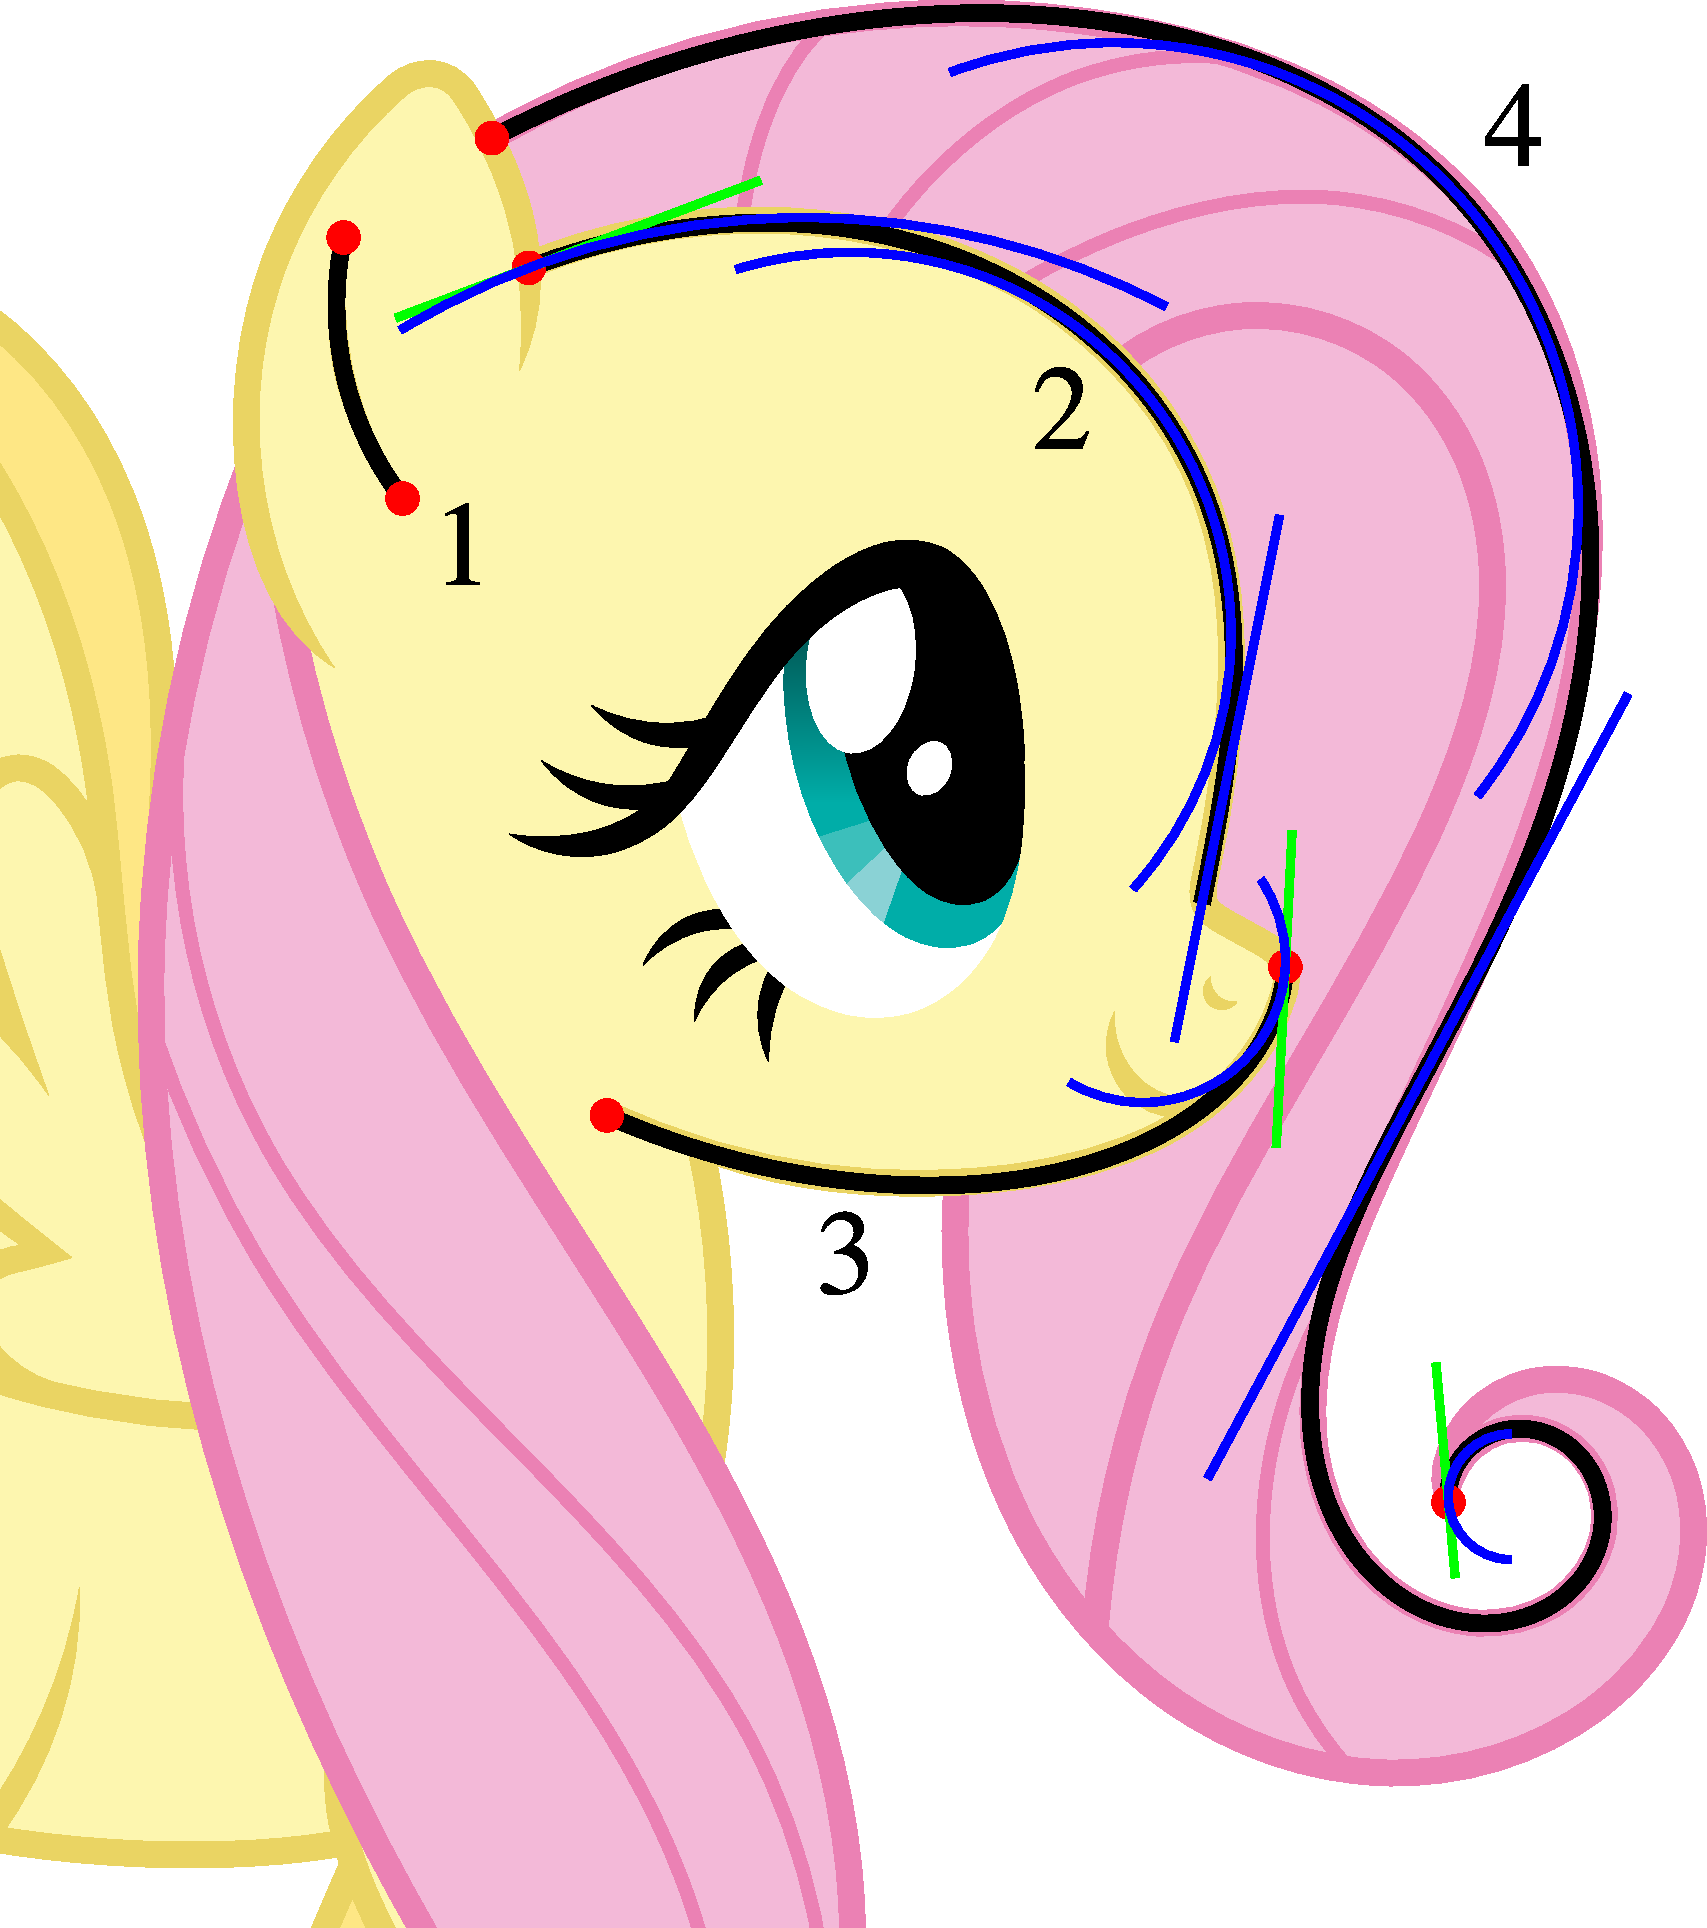
\includegraphics[width=\textwidth]{content/output/examples_prototype_fluttershy.pdf}
					\caption{Fluttershy \cite{fluttershy}}
					\label{figure:examples_prototype_fluttershy}
				\end{subfigure}%
				\begin{subfigure}[b]{5 \textwidth / 13}
					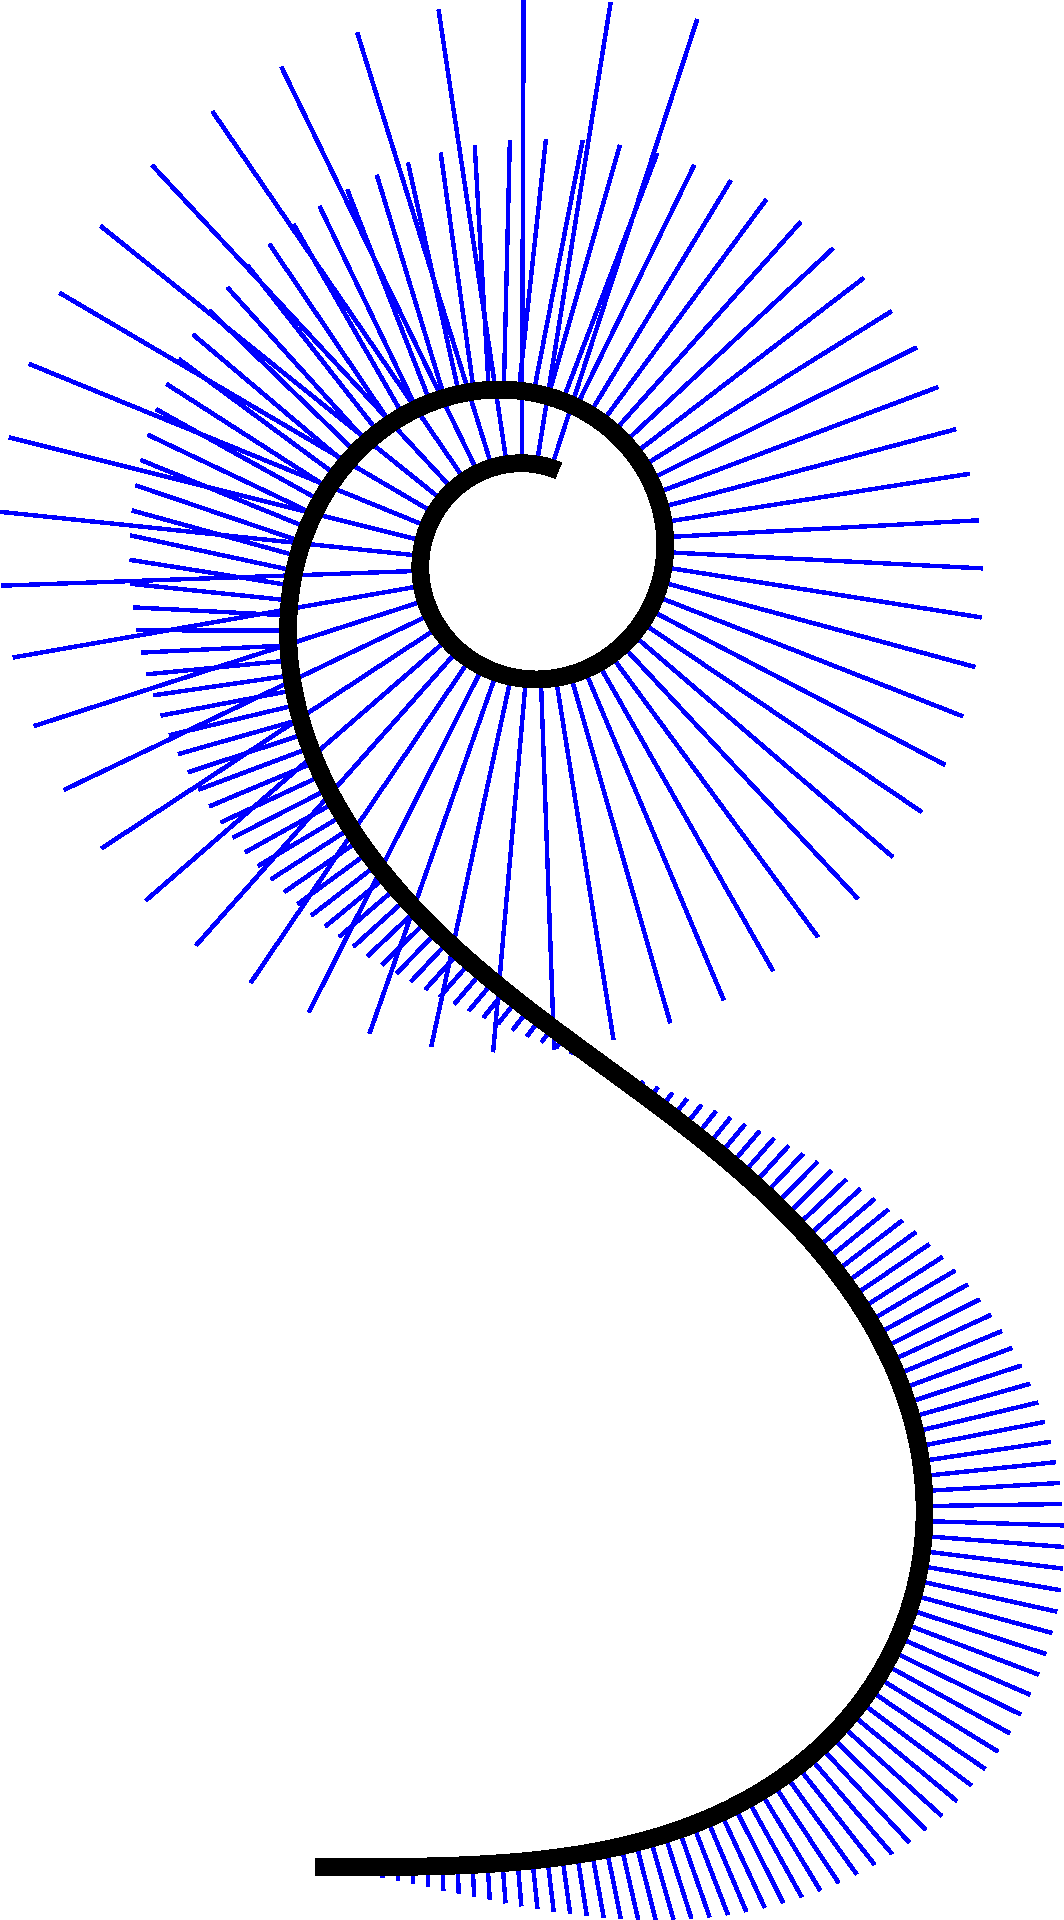
\includegraphics[width=\textwidth]{content/output/examples_prototype_fairness.pdf}
					\caption{Fairness Measure Example}
					\label{figure:examples_prototype_fairness}
				\end{subfigure}
				\caption{Examples of curves designed using the prototype curve design tool. Point specification items are displayed as red dots, direction specification items are displayed green tangent lines and curvature specification items are displayed using blue circular arcs taken from the osculating circle, or blue tangent lines if the curve is locally a straight line. The thin blue lines visualize the curvature at each point of the curve (longer lines meaning higher curvature).}
				\label{figure:examples_prototype}
			\end{figure}

			Figure \ref{figure:examples_prototype_fluttershy} shows a few curves designed using the prototype curve design tool. Example 1 demonstrates how adjusting the arc length of an otherwise unconstrained curve allows the convenient creation of circular arcs between two points.

			Examples 2, 3 and 4 show how to make use of the high expressiveness of the description language. In example 2, the curve is described mainly using three curvature specification items, the point specification item and the direction specification item acting merely as a fixture for the curve, since the curvature specification items leave it unconstrained with regard to translation and rotation. This way, the curve is basically defined by its length and the three curvature specification items, giving the fairness measure maximal freedom controlling the curve. In this case, this enables the fairness measure to establish linearly changing curvature between each pair of curvature specification items.

			Example 3 also starts out with a position that has all 3 types of specification items attached, but instead of specifying the curvature along the way, opts to use a point specification item to enforce the desired shape, resulting in nonlinear but extremely smooth change of curvature. This technique is useful in cases where either nonlinear change of curvature is desired, or where controlling the curve's shape using only curvature specification items is too tedious. The latter may be the case since little errors in curvature specification items propagate and accumulate along the entire curve, making it hard to get the shape right.

			Example 4 uses a mixture of the techniques used in examples 2 and 3, placing curvature specification items along the curve in order to not unnecessarily restrict the fairness measure's freedom and using a final point specification item at the end of the curve to force it into place. This approach ensures that no unintentional bumps are introduced (which can happen easily when placing point specification items in the middle of a curve), while still avoiding the tedious placing of perfectly adjusted curvature specification items (which would be necessary if the final point specification item was not there).

			It may also be worth estimating the amount of information given in the description. Recall that the curve in example 4 was already designed using Bézier splines in section \ref{section:bézier_splines}, using 7 nodes and 12 handles, and Spiro splines in section \ref{section:spiro_splines}, using 7 control points. Here, it is designed using 2 point specification items, 1 direction specification item, 3 curvature specification items and specified arc length. Unfortunately, it is somewhat difficult to directly compare these numbers since specification items use fractions of the arc length for positioning instead of node/control point ordering, as is the case with Bézier splines and Spiro splines. Fraction of arc length positions do of course contain more information than simple orderings, although this is arguably not the case if said positions lie exactly on the start or end of the curve. Furthermore, direction and curvature specification items only specify a scalar value instead of a plane vector, so they could be considered to only supply half as much information as a point specification item. Thus, there is 1 scalar value for arc length, 4 scalar values for points, 1 for directions and 1 for curvatures specified at the start or end of the curve, and 4 scalar values for curvatures specified in the middle of the curve, giving a total of 11 scalar values for the entire specification. This is just short of the 14 scalar values used in the Spiro spline example and a lot less than the 33 scalar values used in the Bézier spline example (where the loss of one degree of freedom for smooth nodes with colinear velocities has already been taken into account). Of course these comparisons cannot be taken as precise, quantitative measurements of conciseness, but they are useful as a coarse judgment of the amount of information that needs to be supplied to define a specific curve.

			Finally, figure \ref{figure:examples_prototype_fairness} demonstrates the ability of the MVC fairness to construct aesthetically pleasing, smooth curves. The indicators for the specification items were left out in this example to make it easier to judge the curve's smoothness.

	\section{Conclusion}
	\label{section:conclusion}

		Having analyzed the usability both through theoretical analysis and experimentally using the prototype curve design tool, we think that the chosen description language looks promising. The added expressiveness has certainly proven useful, facilitating the succinct description of curves which, when using conventional curve design tools, are hard to design and/or lack smoothness due to unfitting description languages.

		While we are very satisfied with the MVC fairness measure, we feel that the specification language can still be improved, for instance by making the specification of the curve's total arc length as well as the specification items' positions optional. Another possible extension would be to allow specification items to be slightly violated in order to improve the curve's fairness (soft specifications). Further experiments using improved versions of the current description language and the prototype curve design tool are needed to make an informed decision. It would also be advisable to do empirical studies with users of vector graphics software to assess the usability of description languages.

		We observe that the prototype curve design tool's usability is still somewhat impaired by performance and stability issues which stem from the use of optimization for solving the problem of curve derivation. Once the final decisions on the description language have been made, some research into how curve derivation can be made more stable and efficient is in order.

		Ideally, the final step of this research would be the incorporation of the developed curve design tool into vector graphics software. The vector graphics editor Inkscape would be a good candidate, mainly because it is free software and thus easy to extend, both technically and from a political/licensing perspective.

	\clearpage

	\appendix

	\section{Definitions}
	\label{section:definitions}

		This section contains definitions used in the rest of the document.

		\subsection{Plane Vectors}
		\label{section:plane_vectors}

			A few basic definitions about vectors in the euclidean plane are needed:
			\begin{align*}
				\overline{\cdot} & : \function{\R{2}}{\R{2}} & \overline{v}      & = \vectorB{-v_2}{v_1}      && \text{orthogonal vector}\\
				\alpha           & : \function{\R{2}}{\RR}   & \apply{\alpha}{v} & = \apply{\atan2}{v_2, v_1} && \text{polar coordinate angle}
			\end{align*}

		\subsection{Parametric Curves}
		\label{section:parametric_curves}

			Parametric curves are described using functions \(\phi : \function{\unit}{\R{n}}\), called the parametrization function. The represented curve is the image of this function. While there are many ways to parametrize a given curve, that is, represent it using a parametrization function, one is usually interested in those which yield a sufficiently smooth parametrization function, allowing for the convenient description of curve properties using differential geometry.

		\subsection{Parametric Plane Curves}
		\label{section:parametric_plane_curves}

			In the special case of parametric plane curves, that is, parametric curves in the euclidean plane, one can define the following functions:
			\begin{align*}
				\phi    & : \function{\unit}{\R{2}} &                    &                                                && \text{point}\\
				\sigma  & : \function{\unit}{\RR}   & \apply{\sigma}{t}  & = \xn{\apply{\phi'}{t}}                        && \text{speed}\\
				\lambda & : \function{\unit}{\RR}   & \apply{\lambda}{t} & = \integral{0}{t}{\apply{\sigma}{u}}{u}        && \text{covered arc length}\\
				\delta  & : \function{\unit}{\RR}   & \apply{\delta}{t}  & = \apply{\alpha}{\apply{\phi'}{t}}             && \text{direction}\\
				\chi    & : \function{\unit}{\RR}   & \apply{\chi}{t}    & = \frac{\apply{\delta'}{t}}{\apply{\sigma}{t}} && \text{curvature}
			\end{align*}

			Using these definitions, the direction \(\apply{\delta}{t}\) is equal to the tangent angle at the point \(\apply{\phi}{t}\). If the curve is locally a straight line at the point \(\apply{\phi}{t}\), the curvature \(\apply{\chi}{t}\) is equal to \(0\). Otherwise, the curvature \(\apply{\chi}{t}\) is equal (up to sign) to the inverse of the radius of the osculating circle at the point \(\apply{\phi}{t}\).

		\subsection{Continuity}
		\label{section:continuity}

			The first way to define continuity of parametric curves is by simply transferring the notion of continuity from calculus as applied to the parametrization function. This leads to the notion of parametric continuity, denoted by \(\contp{n}\), stating that the \(n\)th derivative of the parametrization function is continuous.

			One may notice that this notion of continuity is a little too strict. A curve may look arbitrarily smooth, while its parametrization does not even have \(\contp{1}\) continuity, since the derivatives of the parametrization function may have discontinuities that do not manifest themselves in the curve that it represents. If that is the case, it is always possible to find a different parametrization of the same curve that does not have these discontinuities. This insight gives rise to the definition of geometric continuity, denoted by \(\contg{n}\), which only requires that there exists a reparametrization of the parametric curve which is \(\contp{n}\) continuous.

			It follows immediately that every parametric curve that is \(\contp{n}\) continuous is also \(\contg{n}\) continuous. Observe that \(\contp{0}\) continuity and \(\contg{0}\) continuity are equivalent, since discontinuities in the parametrization function itself manifest themselves directly in the curve it represents, and thus have to exist in all parametrizations of this curve. In the case of parametric plane curves, using the definitions from section \ref{section:parametric_plane_curves}, one can equate \(\contg{0}\) continuity with \(\phi\) being continuous, \(\contg{1}\) continuity with \(\delta\) being continuous and \(\contg{2}\) continuity with \(\chi\) being continuous.

	\clearpage

	\begin{thebibliography}{}

		\bibitem{thesis-mvc}
			\emph{Minimum Curvature Variation Curves, Networks, and Surfaces for Fair Free-Form Shape Design}\\
			Henry Packard Moreton\\
			University of California, Berkeley, 1992

		\bibitem{thesis-spiro}
			\emph{From Spiral to Spline: Optimal Techniques in Interactive Curve Design}\\
			Raphael Linus Levien\\
			University of California, Berkeley, Fall 2009

		\bibitem{paper-mec}
			\emph{The Curve of Least Energy}\\
			B. K. P. Horn\\
			Massachusetts Institute of Technology, January 1981

		\bibitem{fluttershy}
			\emph{Fluttershy}\\
			Hasbro, Inc.\\
			My Little Pony: Friendship is Magic, 2010

		\bibitem{lugia}
			\emph{Lugia}\\
			Nintendo Co., Ltd.\\
			Pokémon, 1999

	\end{thebibliography}

\end{document}
